\documentclass[11pt]{article}

\usepackage[a4paper,margin=1in]{geometry}
\usepackage{amsmath,amssymb,amsfonts}
\usepackage{graphicx}
\usepackage{subcaption}
\usepackage{multirow}
\usepackage{booktabs}
\usepackage{textcomp}
\usepackage{cite}
\usepackage{url}
\usepackage[hidelinks]{hyperref}
\usepackage{authblk}

\renewcommand\Authfont{\normalsize}
\renewcommand\Affilfont{\itshape\small}
\setlength{\affilsep}{0.5em}

\title{\Large A Hybrid CNN--Ensemble Framework with Multi-Backbone and Statistically Validated Evaluation for Multi-Class Brain Tumor Classification}

\author[1]{Md Al Amin Tokder Shoukhin}
\author[1]{Tasmia Jannat}
\author[1]{Md. Ali Hossain}
\author[1]{Nazmul Haque}
\affil[1]{Department of Computer Science and Engineering, Rajshahi University of Engineering and Technology, Rajshahi-6204, Bangladesh}

\date{}

\begin{document}
\maketitle
\vspace{-2em}
\begin{center}
\small
Corresponding author E-mail: alamintokdercse@gmail.com\\[0.3em]
\textit{This manuscript is a preprint and is currently under review for journal publication.}
\end{center}
\vspace{1em}

\begin{abstract}
Reported accuracy in brain tumor MRI classification is usually based on a single train/test split and a single backbone architecture. A single split cannot show how much a reported number depends on which images happened to land in the test set, and a single backbone cannot show whether a result is specific to one network or holds more generally. This paper addresses both concerns directly. We build a hybrid classification pipeline -- two-stage backbone fine-tuning, class-weighted training, test-time augmentation (TTA), and a soft-voting Random Forest/XGBoost/SVM ensemble on the network's embeddings -- and evaluate it under 5-fold cross-validation across four backbone architectures (EfficientNetB0, ResNet50, DenseNet121, MobileNetV2), each trained and timed under an identical protocol, on a four-class, 7,200-image benchmark (glioma, meningioma, pituitary tumor, no-tumor). ResNet50+TTA reaches the highest mean accuracy, 98.38\% $\pm$ 0.23\%, with DenseNet121+TTA close behind at 98.32\% $\pm$ 0.22\% and the DenseNet121 embedding ensemble reaching 98.00\% $\pm$ 0.34\%; the lightweight MobileNetV2 trains roughly 14\% faster than EfficientNetB0 and 30\% faster than ResNet50, with the lowest inference latency of any backbone tested (less than half DenseNet121's), while still reaching 97.96\% $\pm$ 0.32\% with TTA -- ahead of the original EfficientNetB0 configuration (97.75\% $\pm$ 0.25\%) on both accuracy and every efficiency measure. An exact Wilcoxon signed-rank test over the five paired folds shows that both ResNet50 and DenseNet121 outperform EfficientNetB0 in every single fold ($p=0.031$ each), while MobileNetV2's improvement over EfficientNetB0 does not reach significance at this sample size ($p=0.156$). Test-time augmentation improves accuracy over the plain CNN softmax output for every backbone tested, and this improvement is statistically significant in every case ($p=0.031$). Grad-CAM visualizations further indicate the network attends to anatomically relevant regions rather than incidental artifacts. We report these results, together with their limitations and full computational cost, as evidence for a reliability-oriented, multi-backbone evaluation protocol for MRI-based tumor classification, rather than as a claim of a single new state-of-the-art accuracy figure.
\end{abstract}

\noindent\textbf{Keywords:} Brain Tumor Classification, Convolutional Neural Network, Transfer Learning, Backbone Comparison, Ensemble Learning, Cross-Validation, Statistical Significance Testing, Magnetic Resonance Imaging

\section{Introduction}
\label{sec:intro}

Brain tumors occur when abnormal cells grow uncontrollably inside the brain \cite{r16}. Depending on where the tumor forms, it can affect motor function, memory, or basic cognition. The WHO classification recognizes dozens of distinct tumor types and grades \cite{louis2021who}, but for imaging-based triage, the coarser classification used in this paper -- glioma, meningioma, pituitary tumor, or no tumor -- is still the basis for most automated systems. Early and accurate diagnosis is important because it determines whether treatment can be properly planned \cite{r16}. The scale of the problem is large: in the United States alone, the American Cancer Society estimates around 24,820 new malignant brain and CNS tumor diagnoses for 2025, with roughly 18,330 deaths \cite{r4}.

Magnetic Resonance Imaging (MRI) is the most common imaging method for this task because it shows soft tissue detail well and does not require invasive procedures \cite{r16}. However, a radiologist still needs to review the scan and make a diagnosis, which takes time and can vary between readers. Automated tools aim to close this gap by making the diagnosis process faster and more consistent, not by replacing the radiologist \cite{r19}.

Deep learning, especially CNNs, has significantly improved this problem in recent years \cite{r16, r17}. However, medical imaging datasets are usually small compared to what these models typically need, so overfitting remains a common issue \cite{r19}. A common solution is to combine a CNN with a traditional classifier, using the network for feature extraction and a classifier such as Random Forest for the final decision \cite{r18, r20}. Data augmentation is another common technique used to get more out of a limited dataset \cite{r20}.

Two evaluation issues in this literature motivate this paper. The first is how these methods are evaluated across data splits: many papers report accuracy from only one train/test split, and this number can change a lot depending on which images end up in the test set. Cross-validation, where multiple splits are used and the results are averaged, gives a more reliable estimate, and this is the approach we use throughout this paper. The second, less-discussed issue is architectural: most papers in this space report results for a single backbone network, which leaves open whether a reported accuracy is a property of the overall pipeline (fine-tuning strategy, class weighting, TTA, ensembling) or an artifact of the specific network chosen.

This paper treats both issues as first-class experiments rather than footnotes. The contributions of this paper are as follows:

\begin{enumerate}
    \item We evaluate a hybrid two-stage fine-tuning, TTA, and embedding-ensemble pipeline under 5-fold stratified cross-validation on a four-class, 7,200-image brain tumor MRI dataset, reporting mean and standard-deviation accuracy instead of a single train/test split number.
    \item We repeat this evaluation across four backbone architectures (EfficientNetB0, ResNet50, DenseNet121, MobileNetV2) under an identical protocol, to test whether reported gains are pipeline-level or backbone-specific, and to characterize the accuracy--latency--training-cost trade-off across backbones.
    \item We verify that the observed improvements from TTA, the embedding ensemble, and the stronger backbones are statistically significant using an exact Wilcoxon signed-rank test on the fold-wise accuracy scores, rather than relying on mean accuracy alone.
    \item We use Grad-CAM to check, qualitatively, whether the network's predictions are anchored to anatomically relevant regions of the MRI slice rather than incidental artifacts.
\end{enumerate}


\section{Related Work}
\label{sec:related}

CNNs have been widely used for brain tumor classification because they can extract hierarchical features from an MRI slice without manual feature engineering. Dorfner et al. \cite{r16} were among the early groups to show this works well for both segmentation and classification, with the aim of reducing the subjectivity of manual review. Kaifi \cite{r17} used a modified softsign activation function and reported 97.6\% accuracy on the same four-class glioma/meningioma/pituitary/no-tumor problem used in this paper. Both works show CNNs are useful for this task, but they also face two common limitations: limited interpretability and a constant need for more labeled data than these datasets usually provide.

A common solution to the labeled-data problem is combining CNNs with traditional classifiers instead of relying only on the network's own output. Al-Zoghby et al. \cite{r18} used a dual-CNN classifier published in \emph{Diagnostics} and reported 97.3\% accuracy. Vision Transformers \cite{dosovitskiy2021vit} have also become a popular alternative, mainly because they can model long-range spatial relationships that convolutions may miss. Karagoz et al. \cite{r19} combined a Residual Vision Transformer with self-supervised pretraining to address limited labels, which is reasonable given how small most public brain tumor datasets are. G\'omez-Guzm\'an et al. \cite{gomezguzman2025swin} benchmarked several pretrained CNNs and transformer backbones on the same Kaggle dataset identifier used in this paper (a 7,023-image release, versus the 7,200-image, exactly class-balanced release used here; Section~\ref{sec:limitations}), and a Swin-Tiny transformer reached 99.24\% on a single 75/25 split. This shows that transformer backbones are increasingly competitive with CNNs on this problem, although, like most results in this comparison, the number comes from a single split rather than cross-validation, and from a single backbone rather than a systematic comparison.

Ensemble methods and augmentation techniques are also common in this area. Talukder et al. \cite{r20} combined contrast-enhancement preprocessing with an Inception V3-based transfer learning ensemble and reported 98.89\% accuracy across glioma, meningioma, and pituitary tumor. Standard augmentation techniques -- rotation, flipping, and increasingly GAN-based synthesis \cite{goodfellow2014gan} -- are commonly used to expand small datasets, and self-supervised pretraining on unlabeled scans has also become popular for the same reason, especially since transfer learning from ImageNet-scale pretraining has been shown to transfer well to medical imaging despite the domain gap \cite{morid2021transfer}.

Two limitations are common across this literature. First, interpretability is often not addressed directly -- Grad-CAM and similar attention-based explanations are usually mentioned as future work rather than actually reported. Second, a large number of these studies report accuracy from a single train/test split rather than cross-validation, making it difficult to know how much of the reported accuracy reflects real performance versus split-specific variance. This is a broader methodological issue that has been flagged across medical imaging machine learning in general, not just this subfield \cite{varoquaux2022leakage}. Relatedly, almost none of these studies report results for more than one backbone architecture under an identical training and evaluation protocol, so it is generally unclear how much of a reported result would transfer to a different, equally reasonable choice of network.

Table~\ref{tab:related_work} summarizes the studies discussed above alongside the evaluation protocol each one used. With the exception of G\'omez-Guzm\'an et al. \cite{gomezguzman2025swin}, none of these studies report a cross-validated accuracy, and none compare more than one backbone under a controlled protocol. These are the two gaps Section~\ref{sec:methodology} addresses directly.

\begin{table}[htbp]
\centering
\caption{Summary of related work on this and closely related four-class/three-class brain tumor MRI benchmarks, and the evaluation protocol each study used.}
\label{tab:related_work}
\small
\begin{tabular}{@{}p{2.6cm}p{3.2cm}p{1.6cm}p{3.4cm}@{}}
\toprule
\textbf{Study} & \textbf{Model} & \textbf{Accuracy} & \textbf{Protocol} \\
\midrule
Dorfner et al. \cite{r16} & CNN (review) & -- & Not applicable \\
Kaifi \cite{r17} & CNN, modified softsign & 97.6\% & Single split, one backbone \\
Al-Zoghby et al. \cite{r18} & Dual-CNN & 97.3\% & Single split, one backbone \\
Karagoz et al. \cite{r19} & ResViT + SSL & 98.47\% & Single split, one backbone \\
Talukder et al. \cite{r20} & Inception V3 ensemble & 98.89\% & Single split, one backbone \\
G\'omez-Guzm\'an et al. \cite{gomezguzman2025swin} & Multiple CNNs + Swin-Tiny & 99.24\% (best) & Single 75/25 split, multiple backbones \\
\textbf{This study} & EfficientNetB0/ResNet50/ DenseNet121/MobileNetV2 + TTA / embedding ensemble & \textbf{98.38\%} (best backbone, 5-fold mean) & 5-fold CV, 4 backbones \\
\bottomrule
\end{tabular}
\end{table}


\section{Methodology}
\label{sec:methodology}

This study establishes a systematic machine learning framework for multi-class brain tumor classification, structured around two linked experiments: (i) a multi-backbone, cross-validated comparison of the hybrid pipeline, and (ii) statistical validation of the resulting gains.

\subsection{Dataset Description}
\label{sec:datasets}

This study uses a four-class brain tumor MRI dataset containing 7,200 images: 1,800 each of glioma, meningioma, pituitary tumor, and no-tumor. Direct inspection (Section~\ref{sec:eda}) confirms the dataset is exactly class-balanced. Some prior works using the same Kaggle dataset identifier report a total of 7,023 images with an imbalanced, smaller no-tumor class, which most likely reflects an earlier release of the dataset rather than the snapshot used here; Section~\ref{sec:limitations} discusses what this means for the benchmarking comparison in Section~\ref{sec:sota}. Table~\ref{tab:datasets} summarizes the operational characteristics of the dataset actually used in this paper.

\begin{table}[htbp]
\centering
\caption{Operational characteristics of the dataset used in this study.}
\label{tab:datasets}
\small
\begin{tabular}{@{}p{3.2cm}p{6.6cm}@{}}
\toprule
\textbf{Property} & \textbf{Value} \\
\midrule
Classes & Glioma, meningioma, pituitary tumor, no-tumor (4) \\
Samples & 7,200 images (1,800 per class) \\
Patients recorded & No \\
Split used & Image-level, stratified 5-fold \\
Backbones evaluated & EfficientNetB0, ResNet50, DenseNet121, MobileNetV2 \\
\bottomrule
\end{tabular}
\end{table}

The dataset is provided as separate Training and Testing folders and does not record a patient or subject identifier for any image. We merge both folders and re-split the combined dataset using stratified 5-fold cross-validation, so that every image is used as test data exactly once. Because no patient identifier is available, this split is performed at the image level; Section~\ref{sec:limitations} discusses what this means for interpreting the resulting accuracy.

\begin{figure}[htbp]
\centering
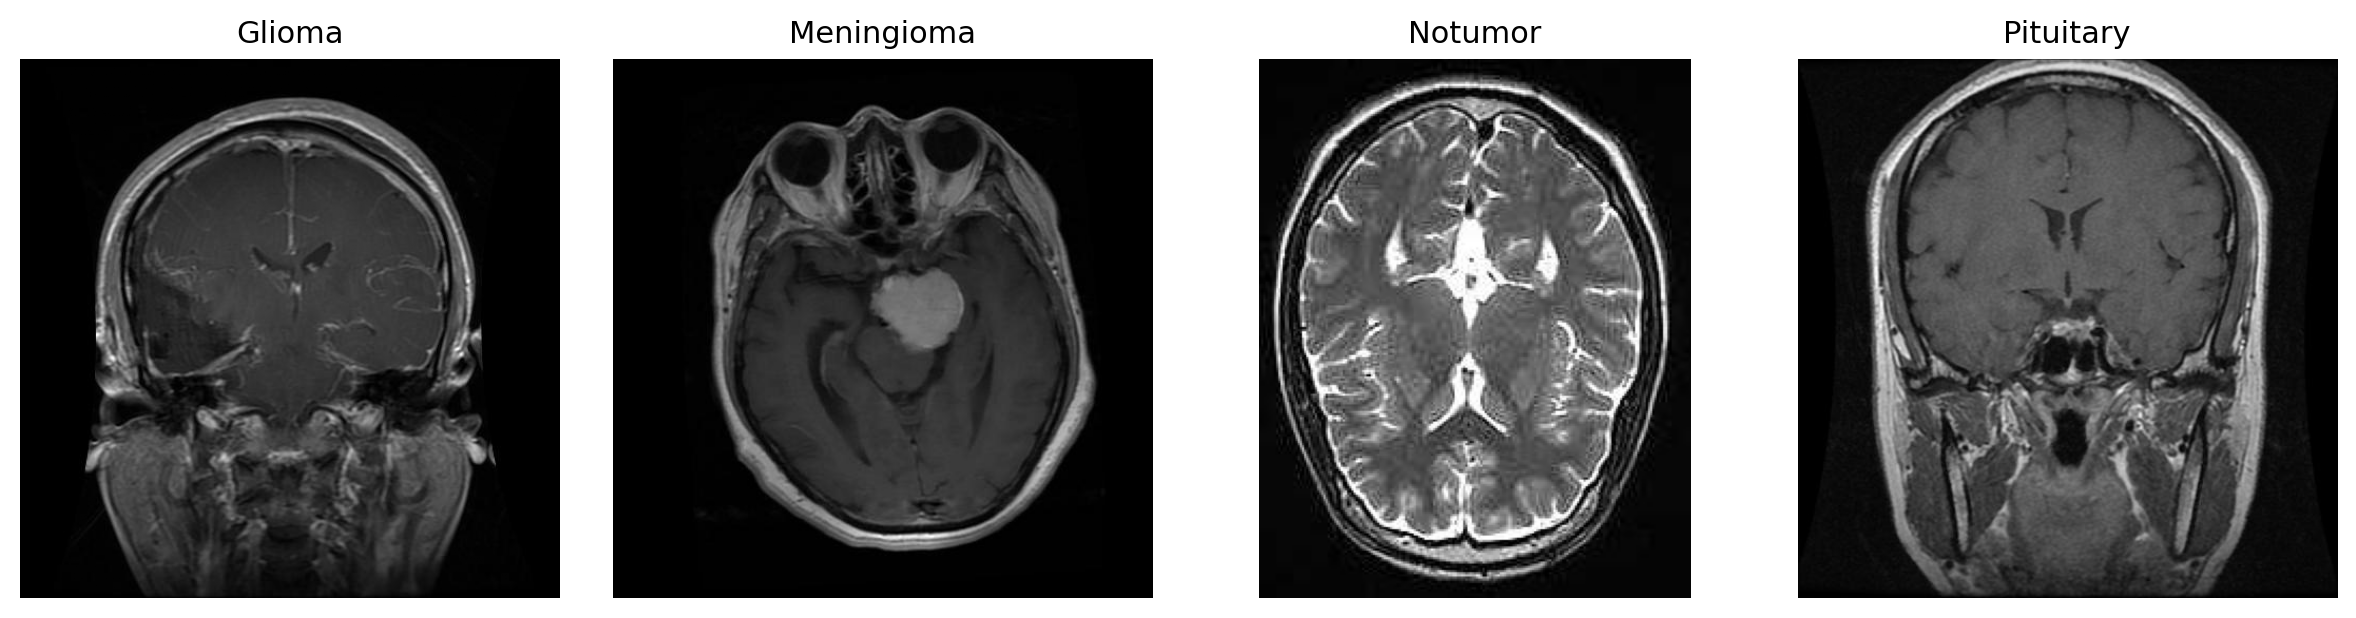
\includegraphics[width=0.55\textwidth]{images/dataset_image.PNG}
\caption{Sample MRI slices from the four-class brain tumor dataset.}
\label{figure_1}
\end{figure}

\subsection{Exploratory Data Analysis}
\label{sec:eda}

Before training any model, we characterize the dataset directly rather than assuming it matches how it is usually described in prior work: class balance, image dimensions, per-class pixel intensity, and a visual check of what each class typically looks like. Figure~\ref{fig:eda_class} confirms the class distribution is exactly balanced at 1,800 images per class, which is itself a departure from the imbalanced count reported for this dataset in some prior work (Section~\ref{sec:limitations}). Figure~\ref{fig:eda_dims} shows that image dimensions are not perfectly uniform across the merged dataset (a bimodal cluster around 220 and 512 pixels, with a long tail up to 1,446 pixels), which is why every image is explicitly resized to 224$\times$224 during preprocessing (Section~\ref{sec:preprocessing}) rather than assumed to already match. Figure~\ref{fig:eda_samples} shows five representative images per class; it also makes visible two things not captured by the summary statistics alone: images within a single class are not all the same anatomical plane (axial, coronal, and sagittal views are mixed together within every class), and at least one no-tumor example is visibly a CT scan rather than an MRI slice (a bright skull ring against a dark interior, unlike the T1-weighted MRI contrast seen elsewhere), which we flag here rather than only in Section~\ref{sec:limitations} since it directly qualifies the ``T1-weighted'' description applied to the dataset as a whole. Figure~\ref{fig:eda_intensity} shows the distribution of mean pixel intensity per class; unlike what we originally expected, no-tumor slices are visibly and consistently brighter (higher median intensity, tighter spread) than the three tumor classes, which is a real, systematic difference between no-tumor and the tumor classes rather than a null result, and is a plausible contributor to no-tumor consistently being the easiest class to classify correctly (Section~\ref{sec:backbone_results}). Figure~\ref{fig:eda_mean} shows the pixel-wise average image per class: the no-tumor average is visibly sharper and less blurred than the tumor-class averages, consistent with more consistent framing/alignment across no-tumor slices, whereas the tumor classes show more positional variation, which is itself expected given that a tumor's location varies from patient to patient while a healthy slice is more likely to be taken from a standardized anatomical position.

\begin{figure}[htbp]
\centering
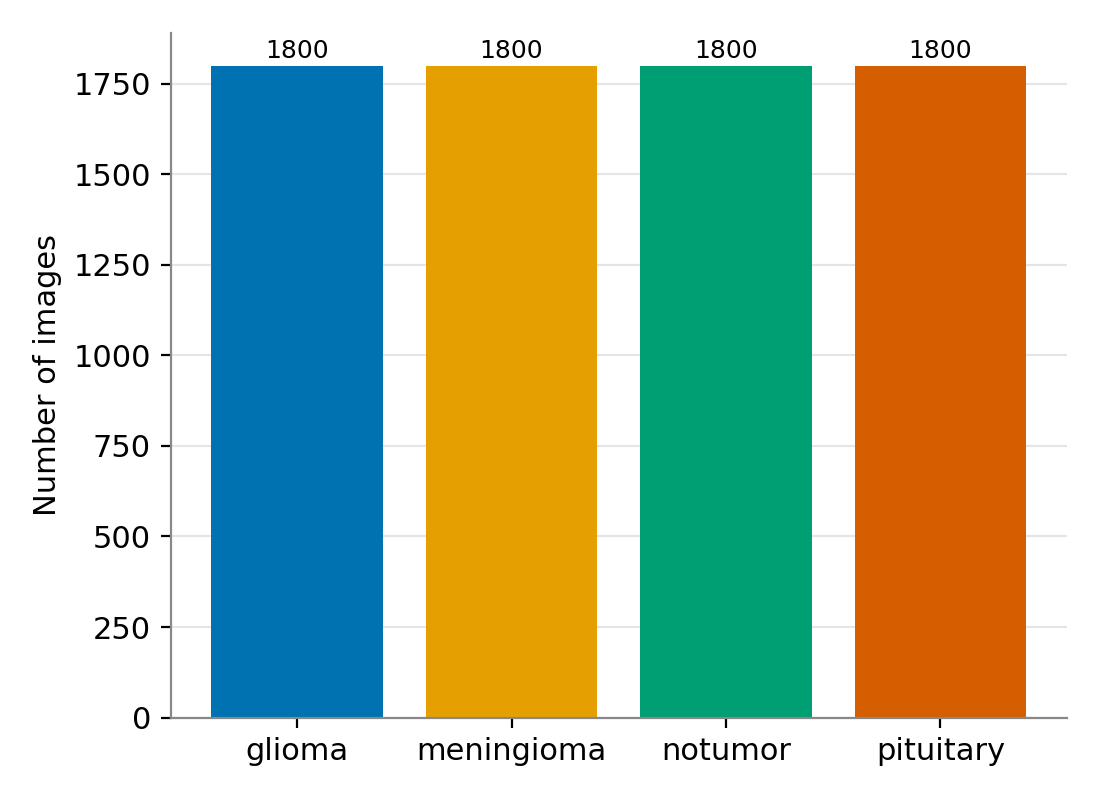
\includegraphics[width=0.48\textwidth]{images/eda_a_class_distribution.png}
\caption{Class distribution across the merged Training and Testing folders.}
\label{fig:eda_class}
\end{figure}

\begin{figure}[htbp]
\centering
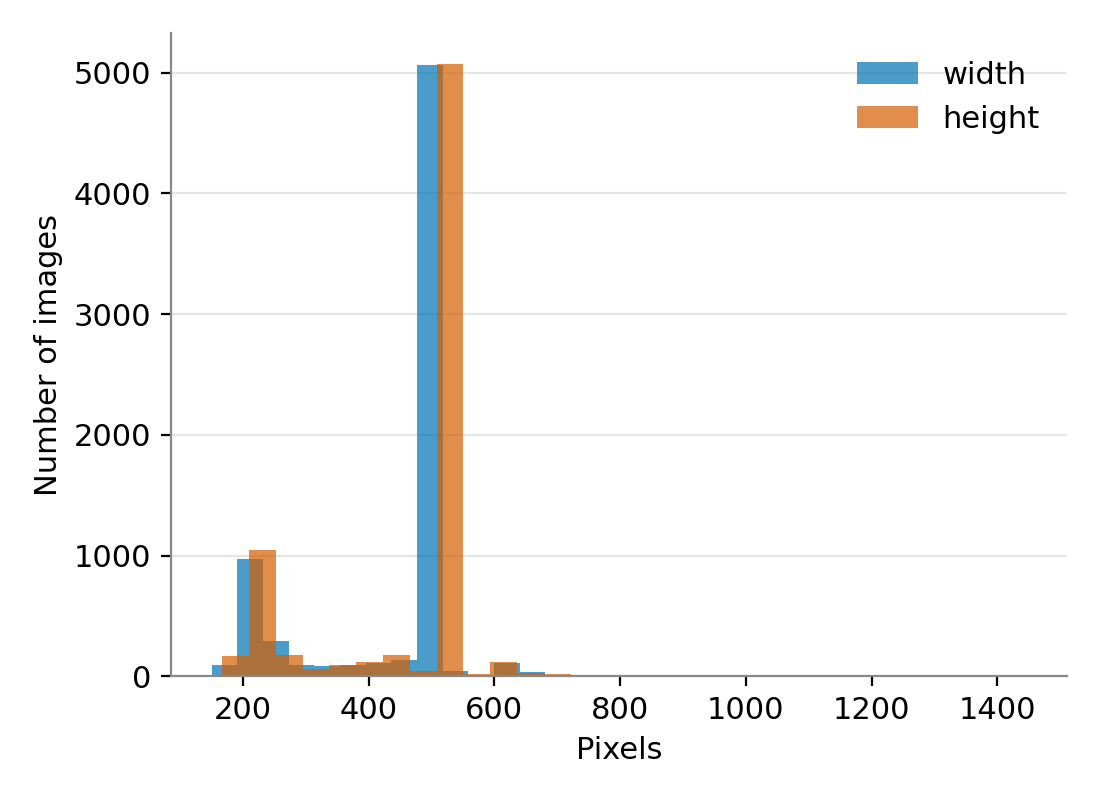
\includegraphics[width=0.48\textwidth]{images/eda_a_image_dimensions.png}
\caption{Distribution of image width and height (pixels) before resizing.}
\label{fig:eda_dims}
\end{figure}

\begin{figure}[htbp]
\centering
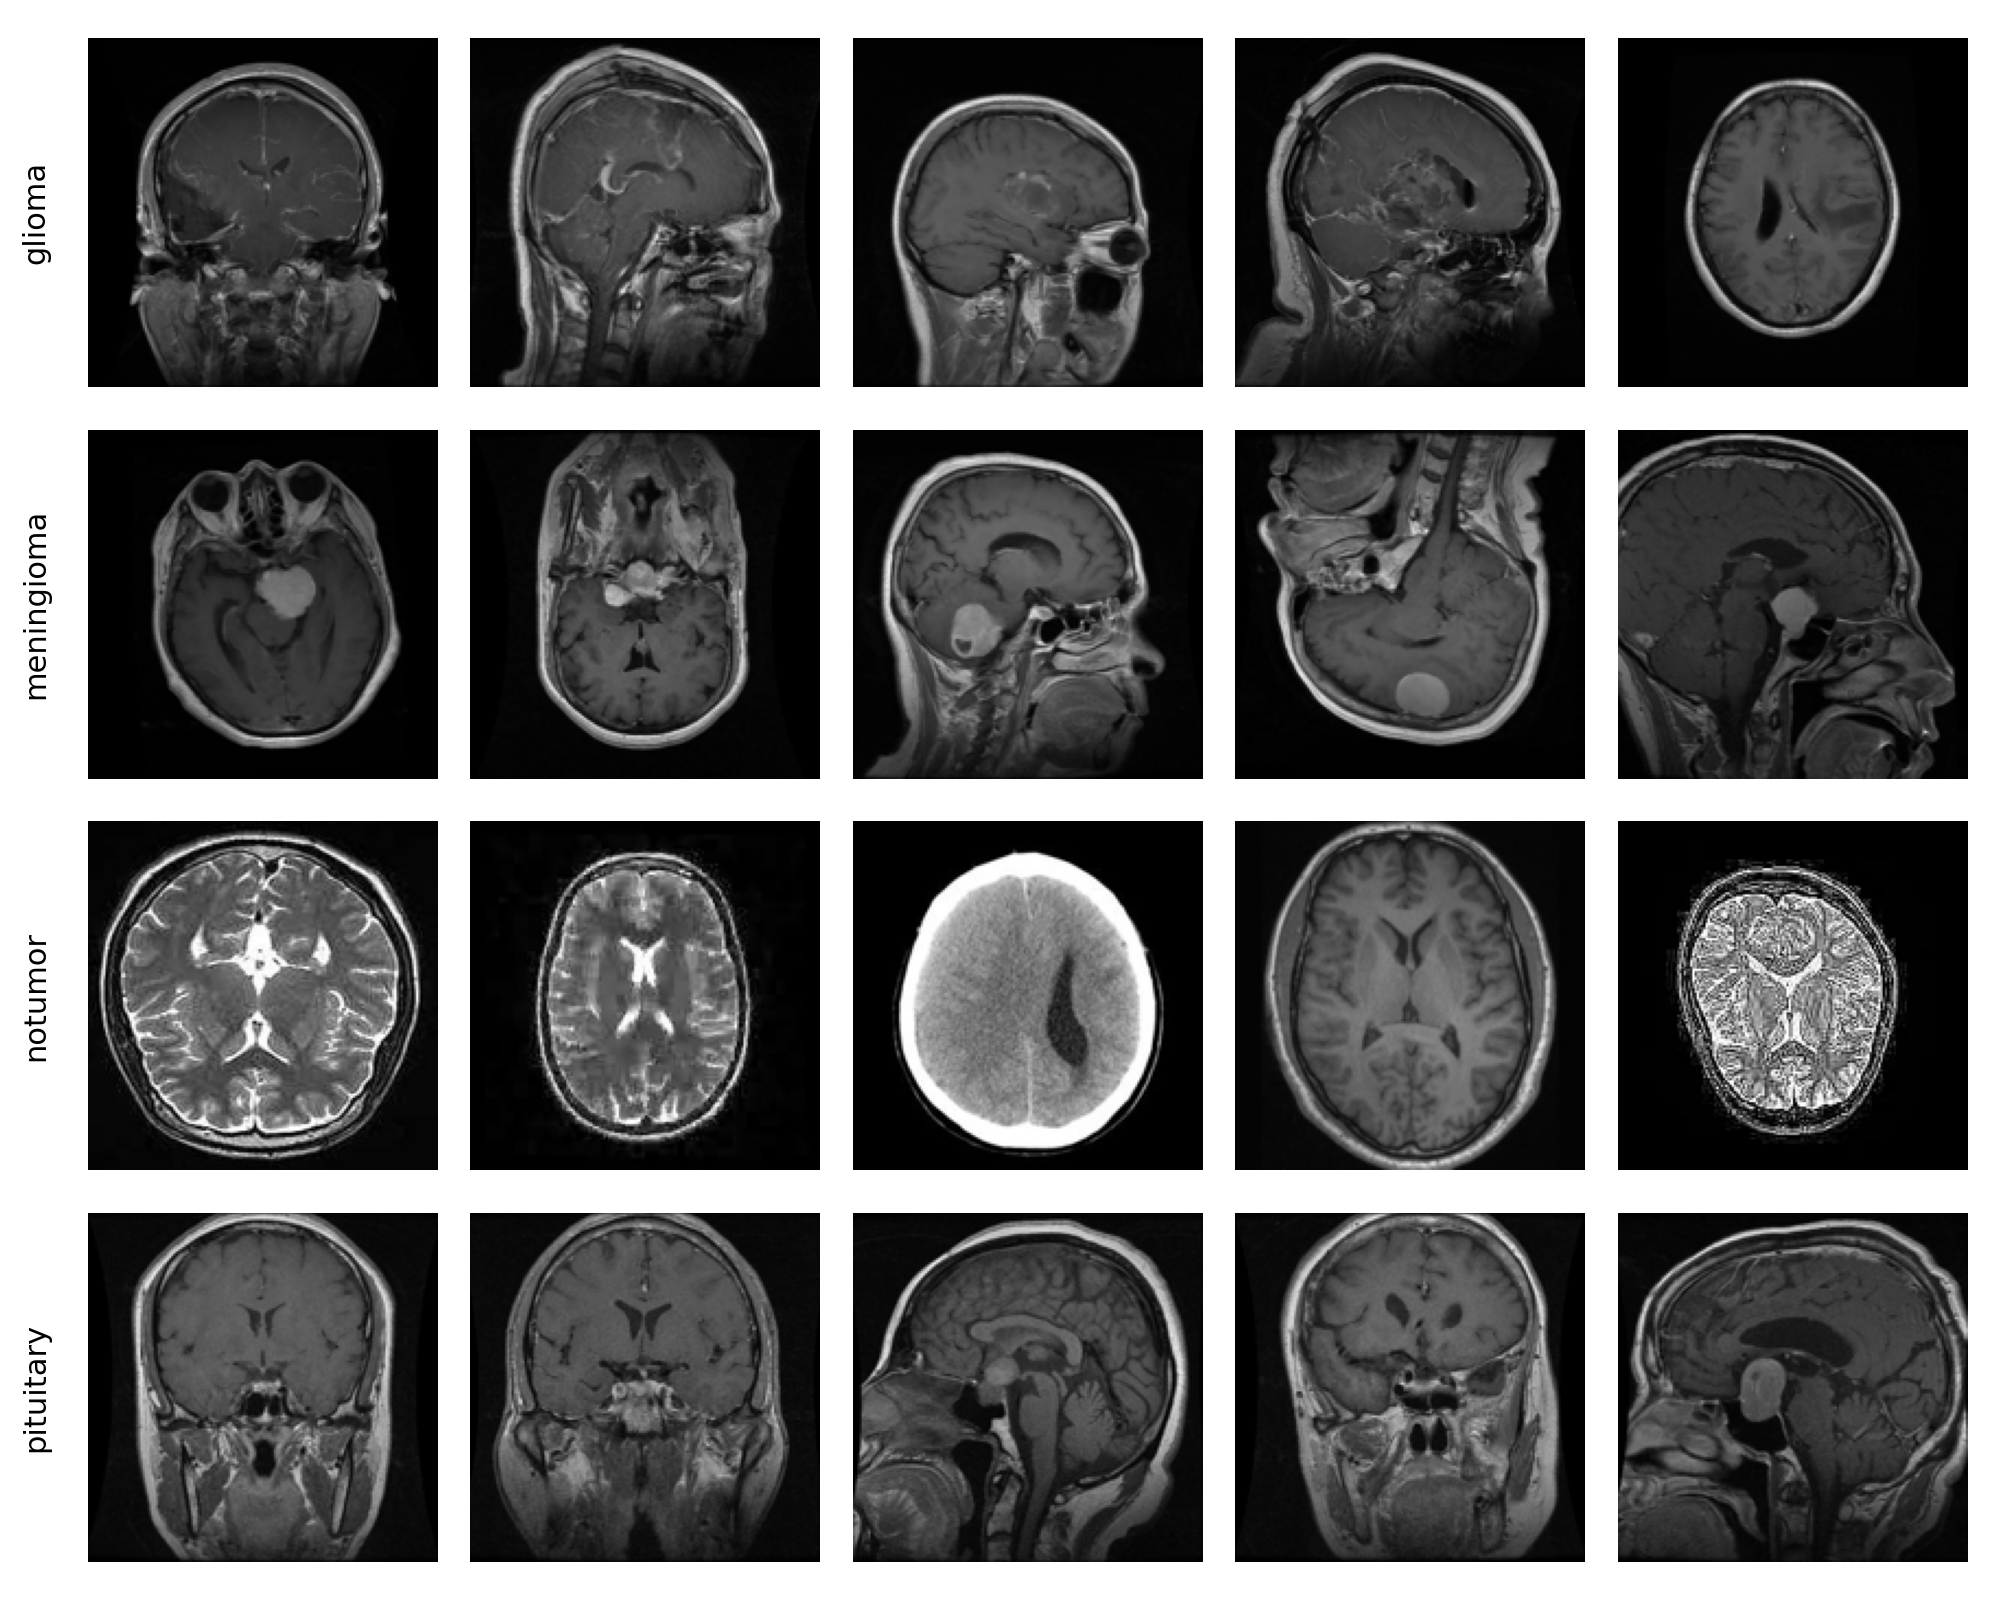
\includegraphics[width=\textwidth]{images/eda_a_sample_grid.png}
\caption{Five representative images per class.}
\label{fig:eda_samples}
\end{figure}

\begin{figure}[htbp]
\centering
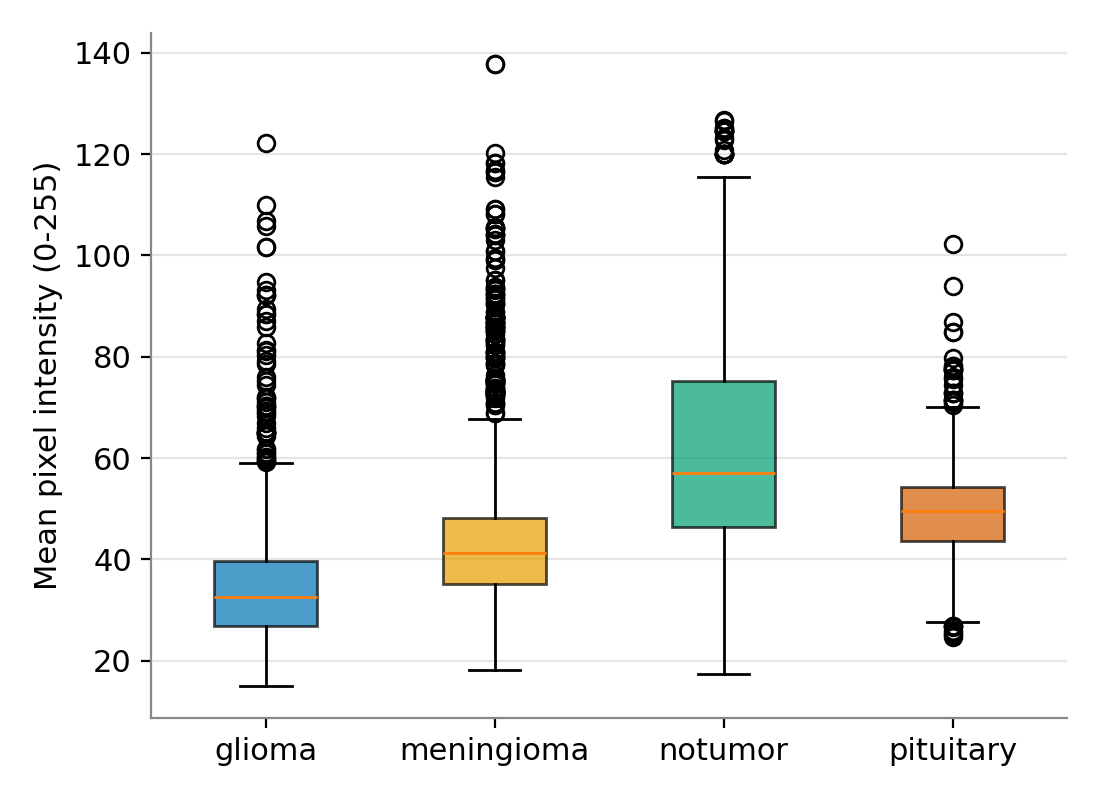
\includegraphics[width=0.48\textwidth]{images/eda_a_intensity_boxplot.png}
\caption{Distribution of mean pixel intensity per image, grouped by class.}
\label{fig:eda_intensity}
\end{figure}

\begin{figure}[htbp]
\centering
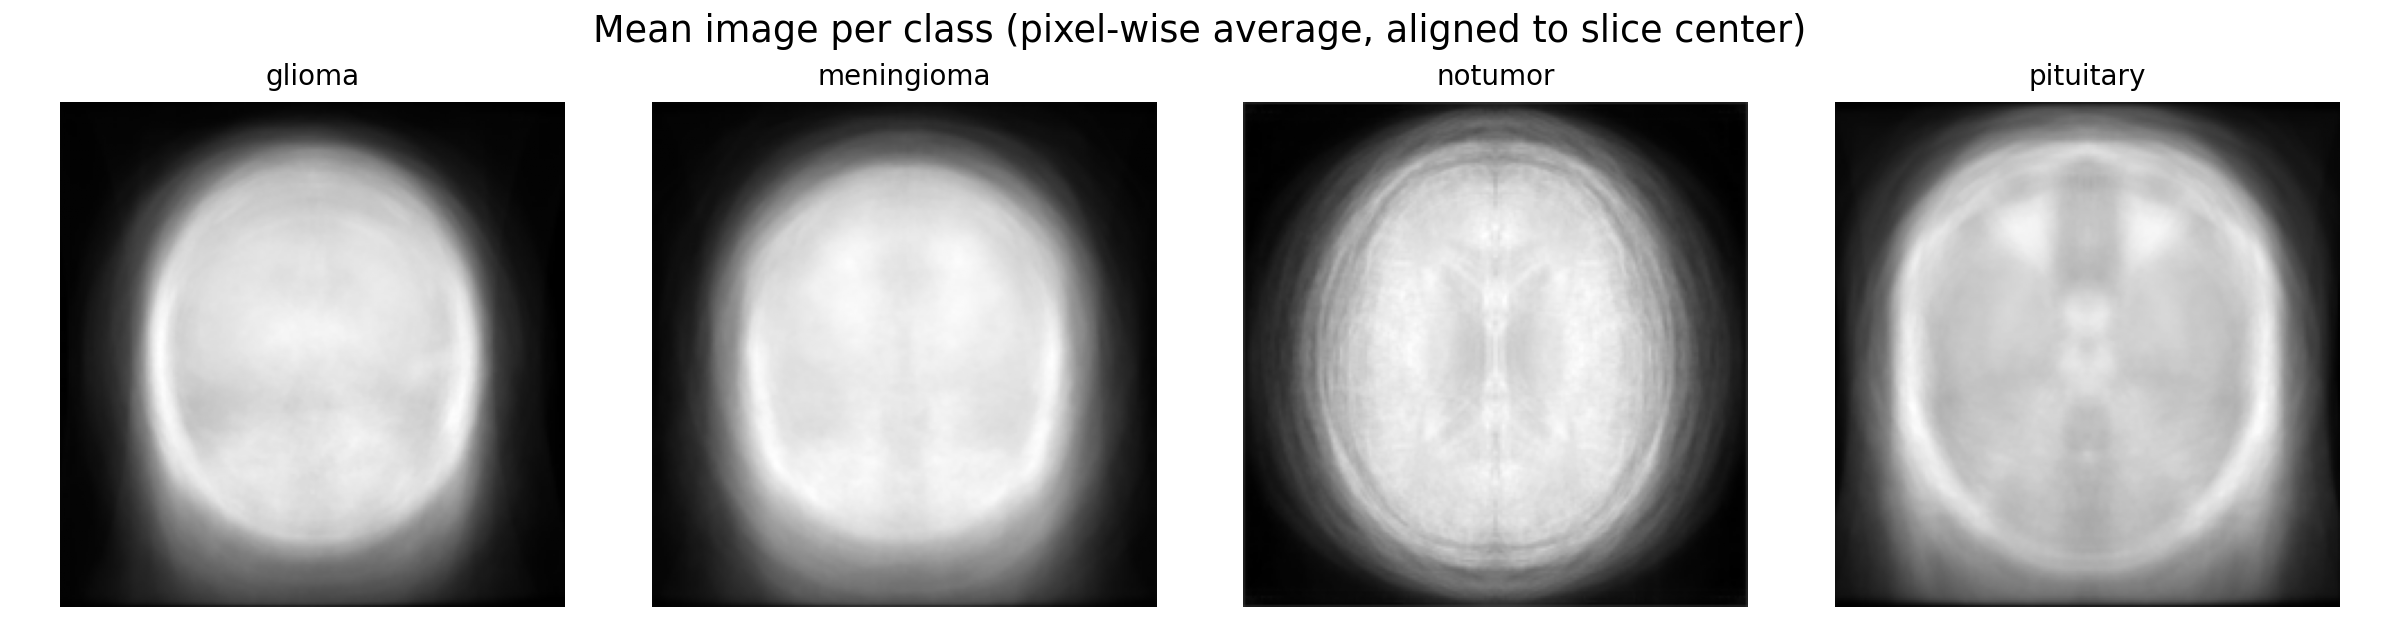
\includegraphics[width=\textwidth]{images/eda_a_mean_images.png}
\caption{Pixel-wise average image per class, computed over every image in that class after resizing to 224$\times$224.}
\label{fig:eda_mean}
\end{figure}

\textbf{Near-duplicate audit.} Section~\ref{sec:limitations} raises subject-level leakage as a concern for this dataset, since it has no patient identifier and is itself a merge of several public sources. We attempted to test for this directly using a 64-bit average-hash Hamming-distance scan (each image downsampled to an 8$\times$8 grayscale thumbnail, thresholded against its own mean). This first attempt failed a basic sanity check and was discarded rather than reported: even at the strictest possible threshold (Hamming distance 0, i.e., an exact hash match), only 49\% of flagged pairs shared the same class label, which is close to the 25\% base rate expected from four balanced classes if the hash carried no signal at all, and far below what a genuine near-duplicate detector should achieve. Manual inspection confirmed the cause: at 8$\times$8 resolution, the hash is dominated by the shared dark-background/centered-oval-skull layout common to all four classes (Figure~\ref{fig:eda_mean}), not by the class-specific content that would distinguish a true near-duplicate pair from two unrelated slices. A corrected two-stage procedure -- using the coarse hash only as a cheap candidate filter, then verifying each candidate pair by direct pixel-level comparison of the resized images -- is a necessary revision to this audit and is left as ongoing work (Section~\ref{sec:limitations}); we report this failure explicitly rather than publish the uncorrected, sanity-check-failing numbers.

\subsection{Preprocessing}
\label{sec:preprocessing}
Each image is decoded, resized to 224$\times$224, and normalized using the preprocessing function that matches each backbone's original ImageNet training regime (Section~\ref{sec:backbones}); using a mismatched normalization silently degrades a backbone's accuracy without raising an error, so this is applied consistently per backbone rather than reusing one backbone's normalization for all four. Although the dataset used in this study turned out to be exactly class-balanced (1,800 images per class; Section~\ref{sec:eda}), we applied class-weighted training rather than assuming balance a priori, since class imbalance is common in this literature and other releases of this dataset are not balanced \cite{buda2018imbalance}. The weights are the inverse class frequency within each training fold, computed using \texttt{sklearn}'s \texttt{compute\_class\_weight} function in \texttt{balanced} mode and applied directly to the loss function; because the classes are balanced here, these weights are approximately uniform and have negligible practical effect on the results in this specific study.

For augmentation, we use a standard set of transformations -- random rotation, translation, zoom, horizontal flip, and contrast jitter -- implemented in a Keras \texttt{Sequential} block. This block is used for two purposes: during training it works as a standard overfitting guard, and during inference the same block is reused for test-time augmentation (Section~\ref{sec:inference}).

\begin{figure}[htbp]
\centering
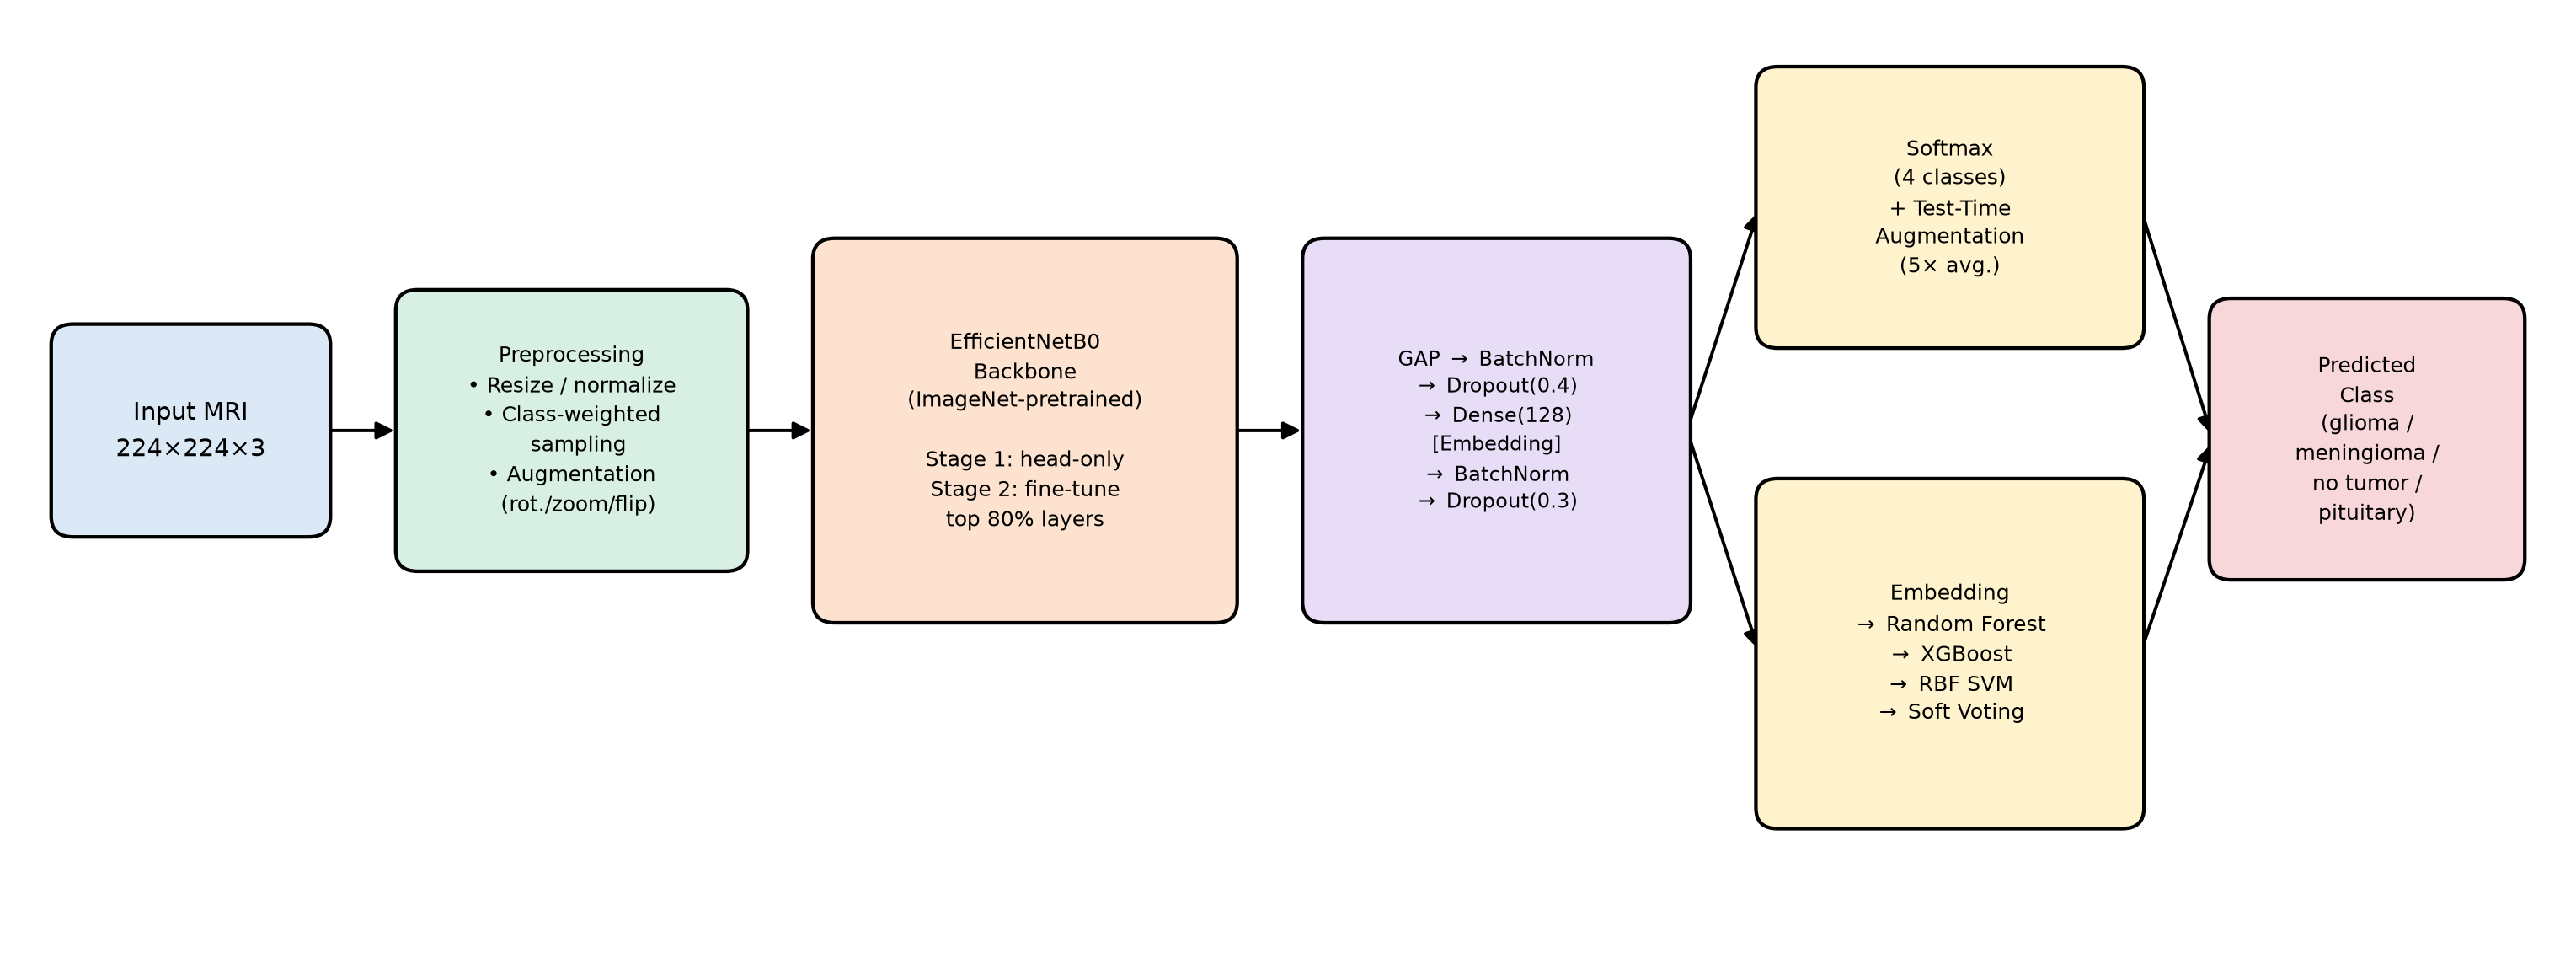
\includegraphics[width=\textwidth]{images/Brain tumor classification.drawio.png}
\caption{Overview of the proposed pipeline: a CNN backbone (one of four compared in this study) with two-stage fine-tuning, followed by two complementary inference heads -- a softmax classifier with test-time augmentation, and a soft-voting ensemble (Random Forest, XGBoost, SVM) trained on the CNN's penultimate-layer embeddings.}
\label{fig:workflow}
\end{figure}

\subsection{Backbone Architectures Compared}
\label{sec:backbones}
Rather than reporting results for a single network, we compare four widely used ImageNet-pretrained CNN backbones under an identical training and evaluation protocol, so that any accuracy difference reflects the backbone rather than a difference in how it was trained or evaluated:

\begin{itemize}
    \item \textbf{EfficientNetB0} \cite{tan2019efficientnet}, the backbone used in our original pipeline, chosen for its compound scaling of depth, width, and resolution, which gives a favorable accuracy--parameter trade-off.
    \item \textbf{ResNet50} \cite{he2016resnet}, a widely used residual architecture that mitigates vanishing gradients in deep networks via identity shortcut connections, included as a strong, well-established baseline.
    \item \textbf{DenseNet121} \cite{huang2017densenet}, which connects each layer to every other layer in a feed-forward fashion, encouraging feature reuse; included to test whether denser connectivity helps on this task.
    \item \textbf{MobileNetV2} \cite{sandler2018mobilenetv2}, a lightweight architecture built on inverted residuals and linear bottlenecks, included to characterize the accuracy--latency trade-off at the low-compute end.
\end{itemize}

For each backbone, we add an identical classification head on top of the backbone's feature output: global average pooling, batch normalization \cite{ioffe2015batchnorm}, dropout (0.4) \cite{srivastava2014dropout}, a 128-unit dense layer that also serves as the embedding for the ensemble described in Section~\ref{sec:inference} (batch-normalized, dropout 0.3), and a final softmax layer. Only the backbone itself and its matching input normalization differ between the four configurations; the head architecture, optimizer, learning rates, epoch budgets, augmentation policy, and cross-validation protocol are held fixed (Section~\ref{sec:cv_protocol}), so that Section~\ref{sec:backbone_results}'s comparison isolates the backbone's contribution.

\subsection{Two-Stage Fine-Tuning}
\label{sec:finetuning}
Training is done in two stages for every backbone. In Stage 1, the backbone is completely frozen and only the new head is trained (Adam \cite{kingma2015adam}, learning rate $10^{-3}$, 8 epochs). This allows the randomly initialized head to stabilize before the pretrained weights are modified. In Stage 2, the top 80\% of the backbone is unfrozen and the whole network is fine-tuned together at a much lower learning rate ($10^{-5}$, up to 35 epochs), with early stopping on validation loss (patience 10) and a reduce-on-plateau schedule (factor 0.5, patience 4). Unfreezing causes a temporary drop in accuracy at the start of Stage 2 for every backbone we tested, which recovers within a few epochs and ends up higher than where Stage 1 alone plateaus.

\subsection{Dual Inference Strategy}
\label{sec:inference}
After the CNN is trained, there are multiple ways to produce a final prediction. We evaluate two of them, for every backbone:

\textbf{Test-time augmentation (TTA).} At test time, each image is passed through the model once without augmentation and 5 additional times using the same augmentations used during training. The resulting softmax outputs are averaged, following an approach used in the uncertainty-estimation literature \cite{wang2019tta}. This adds no additional training cost, only a small increase in inference time, quantified in Section~\ref{sec:efficiency}.

\textbf{CNN-embedding ensemble.} In this approach, the 128-dimensional embedding is extracted from the CNN's penultimate layer (before the softmax) for every image. Three classical models are then trained on this embedding: Random Forest \cite{breiman2001randomforests} (300 trees, balanced class weights), XGBoost \cite{chen2016xgboost} (300 estimators, depth 5, learning rate 0.05), and an RBF SVM (balanced weights, probability outputs enabled). The three models are combined using soft voting. The idea is that the deep network already produces a useful representation of the input, and a small ensemble trained on this representation may add robustness compared to the network's own softmax head.

\subsection{Cross-Validation Protocol}
\label{sec:cv_protocol}
The Training and Testing folders are merged and split into 5 stratified folds, keeping class proportions consistent across folds. Within each fold's training portion, a further 85/15 stratified split is used for validation and early stopping. Every image appears in the test set exactly once across the five folds. Because the dataset does not record a patient identifier, this stratification operates at the image level: it guarantees balanced class proportions per fold, but it cannot guarantee that two slices from the same underlying scan are kept on the same side of a fold, since there is no field in the dataset that would let us group them that way; Section~\ref{sec:limitations} discusses this further. This same 5-fold split (identical random seed, identical fold assignment) is reused for all four backbones, which is what makes the fold-wise comparison in Section~\ref{sec:stats_results} a fair, paired comparison rather than a comparison across different test sets.

We report the mean and standard deviation across the five folds rather than the result of a single run. All training was done on Kaggle using a single Tesla T4 GPU, with batch size 16. Wall-clock training and inference time were measured directly in code for every fold of all four backbones (Section~\ref{sec:efficiency}). As a reproducibility check, we independently re-ran the EfficientNetB0 configuration in a separate Kaggle session, through the same timing-instrumented script used for the other three backbones. The second run's 5-fold mean accuracy (96.01\% CNN, 97.75\% CNN+TTA, 97.26\% ensemble) is close to, but not identical to, the first run's (96.07\%, 97.74\%, 97.36\%; both use the identical fixed random seed and code), with individual folds differing by up to roughly 0.4 percentage points. We attribute this to the well-documented non-determinism of certain cuDNN convolution and reduction kernels on GPU, which a fixed Python/NumPy/TensorFlow random seed does not fully eliminate. We report results from the second, timing-instrumented run throughout this paper for consistency with the other three backbones, and note the run-to-run difference here as a small but real source of variance on top of the fold-to-fold variance already captured by the standard deviations in Table~\ref{tab:backbone_results}.

\subsection{Statistical Significance Testing}
\label{sec:stats_protocol}
Reporting a higher mean accuracy across folds is not, by itself, evidence that the difference is unlikely to be due to chance, particularly with only five folds. To check this, we apply the Wilcoxon signed-rank test \cite{wilcoxon1945} to the fold-wise accuracy scores, treating each fold as a paired observation (e.g., EfficientNetB0's accuracy on fold $k$ versus ResNet50's accuracy on the same fold $k$, which is valid because, as noted in Section~\ref{sec:cv_protocol}, all four backbones share identical fold assignments). We use the Wilcoxon test rather than a paired $t$-test because it does not assume the differences are normally distributed, which is a more defensible assumption with only five paired observations per comparison \cite{demsar2006statistical}. Because $n=5$ is small, we compute the exact one-sided p-value by enumerating all $2^5=32$ possible sign assignments of the ranked differences, rather than using the normal approximation; with this sample size, the smallest attainable one-sided $p$-value is $1/32 \approx 0.031$, which is itself worth keeping in mind when interpreting the results in Section~\ref{sec:stats_results}. We run this test for: CNN vs.\ CNN+TTA and CNN vs.\ the embedding ensemble, for each of the four backbones; and EfficientNetB0 vs.\ each of the other three backbones, and ResNet50 vs.\ DenseNet121.


\section{Results and Discussion}
\label{sec:results}

The evaluation proceeds in the same order as the contributions listed in Section~\ref{sec:intro}: the multi-backbone comparison, statistical validation, computational efficiency, benchmarking against prior work, and interpretability.

\subsection{Multi-Backbone Comparison}
\label{sec:backbone_results}

Table~\ref{tab:backbone_results} reports the mean $\pm$ standard deviation accuracy across the 5 folds for each of the four backbones, under each of the three inference strategies (CNN softmax, CNN+TTA, embedding ensemble). Figure~\ref{fig:backbone_bar} shows the same data as a grouped bar chart.

\begin{table}[htbp]
\centering
\caption{5-fold cross-validation accuracy across four backbone architectures and three inference strategies.}
\label{tab:backbone_results}
\small
\begin{tabular}{@{}lccc@{}}
\toprule
\textbf{Backbone} & \textbf{CNN (softmax)} & \textbf{CNN + TTA} & \textbf{Embedding ensemble} \\
\midrule
EfficientNetB0 & 96.01\% $\pm$ 0.38\% & 97.75\% $\pm$ 0.25\% & 97.26\% $\pm$ 0.27\% \\
ResNet50       & 97.18\% $\pm$ 0.56\% & \textbf{98.38\%} $\pm$ 0.23\% & 97.64\% $\pm$ 0.41\% \\
DenseNet121    & \textbf{97.69\%} $\pm$ 0.53\% & 98.32\% $\pm$ \textbf{0.22\%} & \textbf{98.00\%} $\pm$ 0.34\% \\
MobileNetV2    & 95.04\% $\pm$ 0.72\% & 97.96\% $\pm$ 0.32\% & 96.25\% $\pm$ 0.23\% \\
\bottomrule
\end{tabular}
\end{table}

\begin{figure}[htbp]
\centering
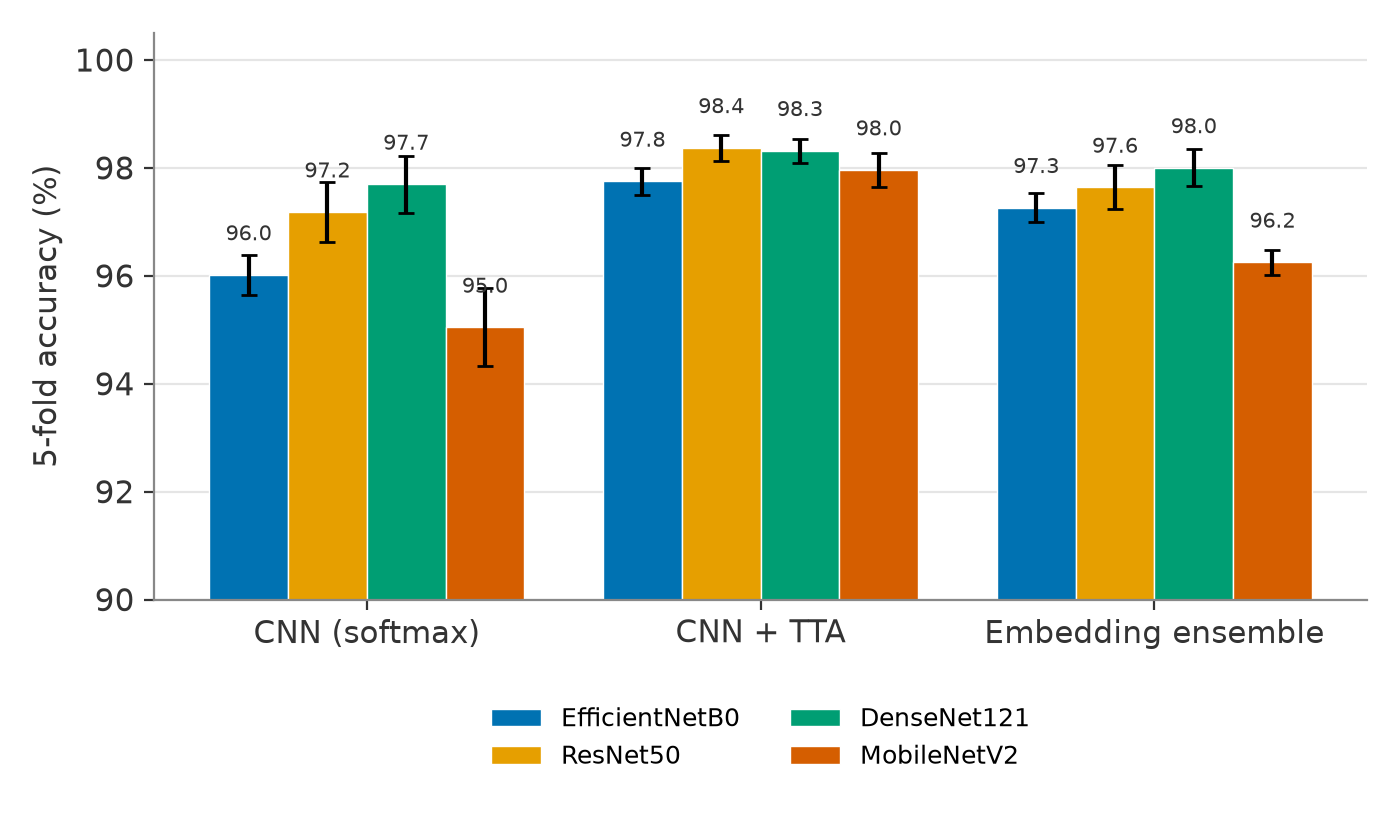
\includegraphics[width=0.85\textwidth]{images/backbone_accuracy_bar.png}
\caption{Mean $\pm$ standard deviation 5-fold accuracy for four backbones under three inference strategies. Error bars show one standard deviation across folds.}
\label{fig:backbone_bar}
\end{figure}

ResNet50 and DenseNet121 both outperform the original EfficientNetB0 backbone on every inference strategy, and DenseNet121 additionally has the lowest fold-to-fold variance for CNN+TTA (0.22\%, versus 0.25\% for EfficientNetB0) while reaching the highest embedding-ensemble accuracy (98.00\%). MobileNetV2's raw CNN softmax accuracy (95.04\%) is clearly the weakest of the four, but TTA closes most of this gap, bringing it to 97.96\%, within 0.4 percentage points of the best backbone despite being the lightest network in the comparison (Section~\ref{sec:efficiency}). Figure~\ref{fig:backbone_variance} shows the per-fold spread for CNN+TTA directly: ResNet50 and DenseNet121's fold-wise accuracies cluster in a narrower, higher band than EfficientNetB0's, while MobileNetV2's folds are more spread out despite a competitive mean.

\begin{figure}[htbp]
\centering
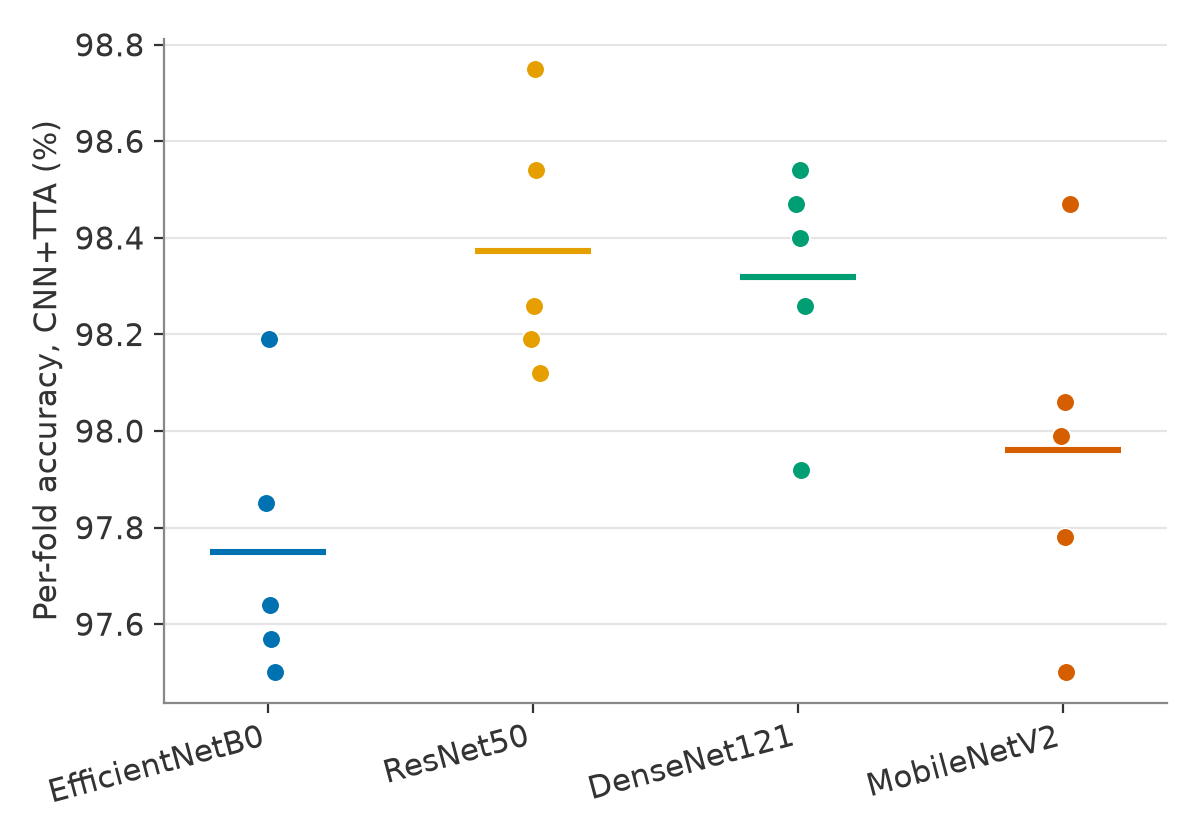
\includegraphics[width=0.7\textwidth]{images/backbone_fold_variance.png}
\caption{Per-fold CNN+TTA accuracy for each backbone. Horizontal bars mark the mean across the five folds.}
\label{fig:backbone_variance}
\end{figure}

Table~\ref{tab:perclass_resnet} shows the per-class results for the single best fold observed in this study (ResNet50, CNN+TTA), and Table~\ref{tab:perclass} shows the corresponding best fold for the original EfficientNetB0 backbone, for direct comparison. In both cases, all four classes -- including no-tumor -- achieve strong results, and the pattern of which class is hardest (meningioma) is consistent across backbones.

\begin{table}[htbp]
\centering
\caption{Representative per-class results, ResNet50 + TTA, best observed fold.}
\label{tab:perclass_resnet}
\small
\begin{tabular}{@{}lcccc@{}}
\toprule
\textbf{Class} & \textbf{Precision} & \textbf{Recall} & \textbf{F1} & \textbf{Support} \\
\midrule
Glioma      & 1.00 & 0.98 & 0.99 & 360 \\
Meningioma  & 0.98 & 0.98 & 0.98 & 360 \\
No Tumor    & 0.98 & 0.99 & 0.99 & 360 \\
Pituitary   & 0.98 & 0.99 & 0.99 & 360 \\
\textbf{Accuracy} & \multicolumn{3}{c}{0.99} & 1440 \\
\bottomrule
\end{tabular}
\end{table}

\begin{table}[htbp]
\centering
\caption{Representative per-class results, EfficientNetB0 + TTA, best observed fold.}
\label{tab:perclass}
\small
\begin{tabular}{@{}lcccc@{}}
\toprule
\textbf{Class} & \textbf{Precision} & \textbf{Recall} & \textbf{F1} & \textbf{Support} \\
\midrule
Glioma      & 0.98 & 0.97 & 0.97 & 360 \\
Meningioma  & 0.97 & 0.99 & 0.98 & 360 \\
No Tumor    & 0.99 & 0.99 & 0.99 & 360 \\
Pituitary   & 0.99 & 0.98 & 0.99 & 360 \\
\textbf{Accuracy} & \multicolumn{3}{c}{0.98} & 1440 \\
\bottomrule
\end{tabular}
\end{table}

Across all five folds and all four backbones, meningioma was consistently the most frequently misclassified class, mostly confused with glioma and pituitary tumor, while no-tumor was consistently the easiest class to classify correctly. This confusion pattern being stable across four otherwise-different backbones suggests it reflects a genuine property of the imaging data (meningioma's variable appearance and less distinct boundaries) rather than an idiosyncrasy of any one network, which we return to in Section~\ref{sec:discussion}.

\subsection{Statistical Significance Testing}
\label{sec:stats_results}

Table~\ref{tab:wilcoxon} reports the exact one-sided Wilcoxon signed-rank test results (Section~\ref{sec:stats_protocol}) for the comparisons of interest.

\begin{table}[htbp]
\centering
\caption{Exact one-sided Wilcoxon signed-rank test results ($n=5$ paired folds per comparison). The smallest attainable $p$-value at this sample size is $1/32 \approx 0.031$.}
\label{tab:wilcoxon}
\small
\begin{tabular}{@{}lc@{}}
\toprule
\textbf{Comparison} & \textbf{One-sided $p$} \\
\midrule
CNN vs.\ CNN+TTA (EfficientNetB0)       & 0.031 \\
CNN vs.\ embedding ensemble (EfficientNetB0) & 0.031 \\
EfficientNetB0 vs.\ ResNet50 (CNN+TTA)  & 0.031 \\
EfficientNetB0 vs.\ DenseNet121 (CNN+TTA) & 0.031 \\
EfficientNetB0 vs.\ MobileNetV2 (CNN+TTA) & 0.156 \\
ResNet50 vs.\ DenseNet121 (CNN+TTA)     & 0.500 \\
CNN vs.\ embedding ensemble (ResNet50)   & 0.031 \\
CNN vs.\ embedding ensemble (DenseNet121) & 0.219 \\
CNN vs.\ embedding ensemble (MobileNetV2) & 0.031 \\
\bottomrule
\end{tabular}
\end{table}

TTA's improvement over the plain CNN softmax output is significant at the $\alpha=0.05$ level for every backbone ($p=0.031$ in each case), consistent with TTA improving accuracy in every single fold we ran. The embedding ensemble's improvement over its own CNN is significant for three of the four backbones (EfficientNetB0, ResNet50, MobileNetV2; $p=0.031$ each), but not for DenseNet121 ($p=0.219$) despite DenseNet121's embedding ensemble having the single highest mean accuracy of any ensemble configuration in Table~\ref{tab:backbone_results} (98.00\%): DenseNet121's own CNN is already strong enough that the ensemble's fold-wise advantage over it is inconsistent in direction. Taken together, these results say the ensemble reliably helps a weaker or moderate backbone, but its marginal value over an already-strong CNN is small and inconsistent enough that five folds cannot distinguish it from chance -- a limitation of statistical power at this sample size, not evidence that the ensemble fails.

For the backbone comparison, both ResNet50 and DenseNet121 beat EfficientNetB0 in every one of the five folds, which is the strongest possible result an exact test can return at $n=5$ and is why both reach $p=0.031$ despite ResNet50 and DenseNet121 having slightly different mean accuracies (98.38\% vs.\ 98.32\%). MobileNetV2, in contrast, beats EfficientNetB0 in only 3 of 5 folds (losing on folds 3 and 4, where EfficientNetB0 happened to have two of its strongest folds), so despite a competitive mean accuracy (97.96\%), its improvement over EfficientNetB0 does not reach significance ($p=0.156$). ResNet50 and DenseNet121 are not significantly different from each other ($p=0.500$, effectively a coin flip across folds). We report exact $p$-values rather than only which comparisons ``pass'' $\alpha=0.05$, because at $n=5$ a result can look decisive (a clean 5/5 sweep) or genuinely ambiguous (a 3/2 split) in a way that the mean accuracy alone does not convey.

\subsection{Computational Efficiency}
\label{sec:efficiency}

Table~\ref{tab:efficiency} reports training time (per fold) and inference latency (per image), measured directly with wall-clock timers around the relevant code for all four backbones under an identical protocol (Section~\ref{sec:cv_protocol}).

\begin{table}[htbp]
\centering
\caption{Computational cost per fold, measured on a single Tesla T4 GPU. Training time is the sum of Stage 1 and Stage 2; inference latency is milliseconds per image.}
\label{tab:efficiency}
\small
\begin{tabular}{@{}lcccc@{}}
\toprule
\textbf{Backbone} & \textbf{Training time} & \textbf{CNN latency} & \textbf{TTA latency} & \textbf{Ensemble latency} \\
\midrule
EfficientNetB0 & 1628.2 s (27.1 min) & 7.02 ms & 28.06 ms & 15.52 ms \\
ResNet50     & 2021.1 s (33.7 min) & 6.42 ms & 35.36 ms & 13.32 ms \\
DenseNet121  & 1796.0 s (29.9 min) & 11.35 ms & 37.67 ms & 11.94 ms \\
MobileNetV2  & 1402.7 s (23.4 min) & 4.50 ms & 23.49 ms & 14.67 ms \\
\bottomrule
\end{tabular}
\end{table}

\begin{figure}[htbp]
\centering
\begin{subfigure}[t]{0.48\textwidth}
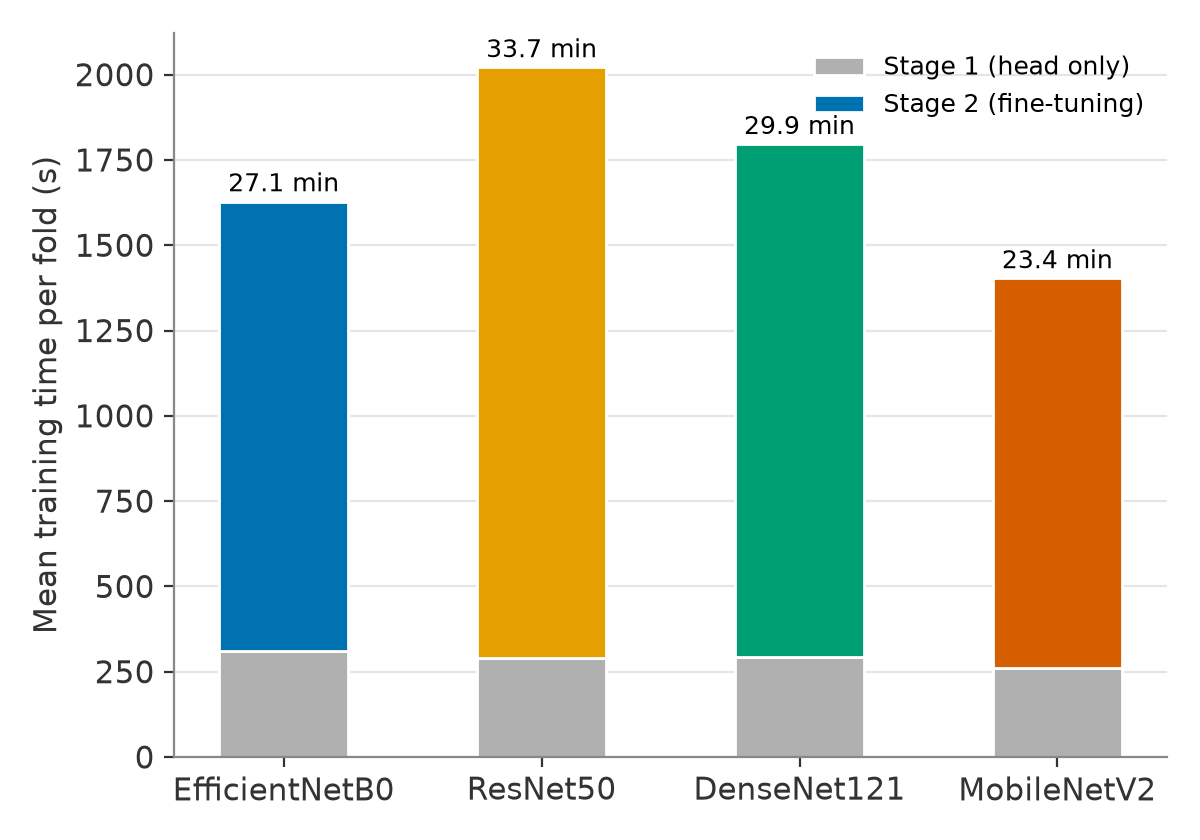
\includegraphics[width=\linewidth]{images/backbone_training_time.png}
\caption{Training time per fold.}
\end{subfigure}
\hfill
\begin{subfigure}[t]{0.48\textwidth}
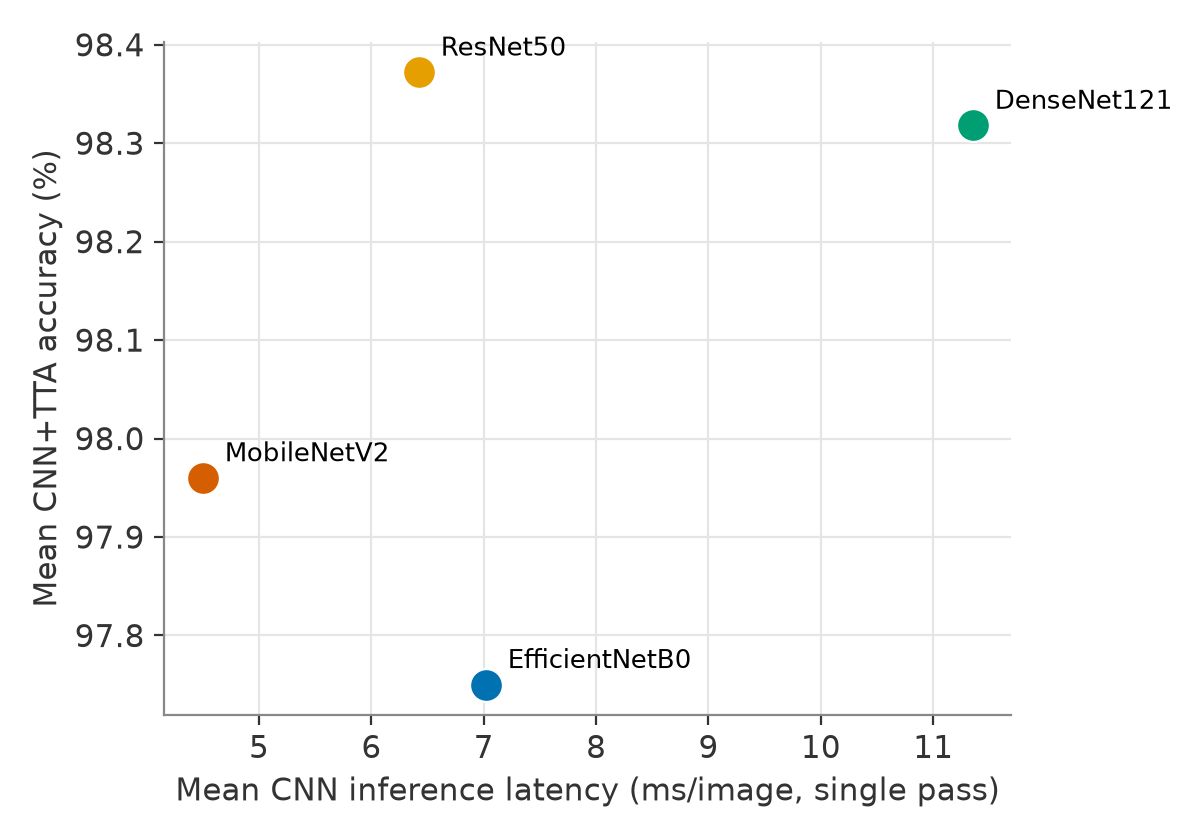
\includegraphics[width=\linewidth]{images/backbone_latency_tradeoff.png}
\caption{Accuracy vs.\ single-pass inference latency.}
\end{subfigure}
\caption{Computational cost of the three timed backbones. MobileNetV2 trains fastest and infers with the lowest latency, at a small accuracy cost relative to ResNet50 and DenseNet121.}
\label{fig:efficiency}
\end{figure}

MobileNetV2 is the cheapest backbone on every axis measured -- roughly 14\% faster to train than EfficientNetB0, 31\% faster than ResNet50, and 22\% faster than DenseNet121 per fold, and its single-pass CNN inference latency (4.50 ms/image) is the lowest of the four, well under half of DenseNet121's (11.35 ms/image) -- while its TTA accuracy (97.96\%) is not only within 0.4 percentage points of the best backbone but is also higher than EfficientNetB0's own TTA accuracy (97.75\%), making MobileNetV2 strictly preferable to the original backbone on both cost and accuracy. TTA inflates latency by roughly 4-6$\times$ over the single-pass CNN for every backbone, since it averages predictions over 5 augmented views plus the clean pass; the embedding ensemble, in contrast, adds only a modest latency overhead over the CNN alone (and is in some cases faster than TTA, since the classical models operate on a 128-dimensional embedding rather than requiring repeated forward passes through the full network). For a deployment setting where inference latency or training cost is a binding constraint, MobileNetV2 with TTA is a clearly reasonable choice; where maximum accuracy is the only consideration, ResNet50 or DenseNet121 with TTA is preferable, at roughly 1.3--1.4$\times$ MobileNetV2's training cost.

\subsection{Comparison with Prior Work}
\label{sec:sota}

Table~\ref{tab:sota_comparison} compares our results with recent papers that used the same or a closely related four-class dataset (the figshare/SARTAJ/Br35H combination). None of these prior papers report a cross-validated mean; they all report single-split accuracy, which, as discussed in Section~\ref{sec:related}, tends to be optimistic and does not indicate how much the result might vary, nor whether it holds for more than one backbone.

\begin{table}[htbp]
\centering
\caption{Comparison with prior work on comparable 4-class brain tumor MRI benchmarks.}
\label{tab:sota_comparison}
\small
\begin{tabular}{@{}p{5.0cm}p{2.3cm}p{2.8cm}@{}}
\toprule
\textbf{Method} & \textbf{Accuracy} & \textbf{Protocol} \\
\midrule
Xception \cite{disci2025advanced} & 95.27\% & Single split \\
Res-BRNet \cite{zahoor2024resbrnet} & 98.22\% & Single split \\
Hybrid CNN--GCN \cite{cnngcn2024hybrid} & 92.91\% & Single split \\
MobileNetV2--SVM \cite{adamu2024mobilenetsvm} & AUC 0.97--1.00\textsuperscript{*} & Single split \\
ResViT + SSL \cite{r19} & 98.47\% & Single split \\
Swin-Tiny (transformer) \cite{gomezguzman2025swin} & 99.24\% & Single split \\
\textbf{Proposed (EfficientNetB0+TTA, 5-fold mean)} & 97.75\% $\pm$ 0.25\% & 5-fold CV \\
\textbf{Proposed (ResNet50+TTA, 5-fold mean)} & \textbf{98.38\%} $\pm$ 0.23\% & 5-fold CV \\
\textbf{Proposed (DenseNet121+TTA, 5-fold mean)} & 98.32\% $\pm$ 0.22\% & 5-fold CV \\
\textbf{Proposed (DenseNet121 ensemble, 5-fold mean)} & 98.00\% $\pm$ 0.34\% & 5-fold CV \\
\bottomrule
\end{tabular}

\vspace{1mm}
{\footnotesize \textsuperscript{*}Per-class AUC reported rather than a single overall accuracy figure; not directly comparable to the accuracy values above.}
\end{table}

Our best configuration, ResNet50+TTA at 98.38\% $\pm$ 0.23\%, is competitive with the strongest single-split numbers in the table (Res-BRNet at 98.22\%, ResViT+SSL at 98.47\%) and is exceeded only by the Swin-Tiny transformer's 99.24\%. Unlike every other row in the table, our numbers come with an error estimate and were obtained across four independent backbone architectures rather than one, which we consider the more meaningful basis for comparison even where our mean is nominally below the single best reported figure.

\subsection{Interpretability: Grad-CAM Visualization}
\label{sec:gradcam}
High accuracy alone does not show whether the model is actually focusing on the tumor or on some unrelated pattern in the image. To check this, we used Gradient-weighted Class Activation Mapping (Grad-CAM) \cite{selvaraju2017gradcam} on the trained EfficientNetB0 network's last convolutional feature map. Fig.~\ref{fig:gradcam} shows one correctly classified example per class with the heatmap overlaid on the original slice.

\begin{figure}[htbp]
\centering
\begin{subfigure}[t]{0.48\linewidth}
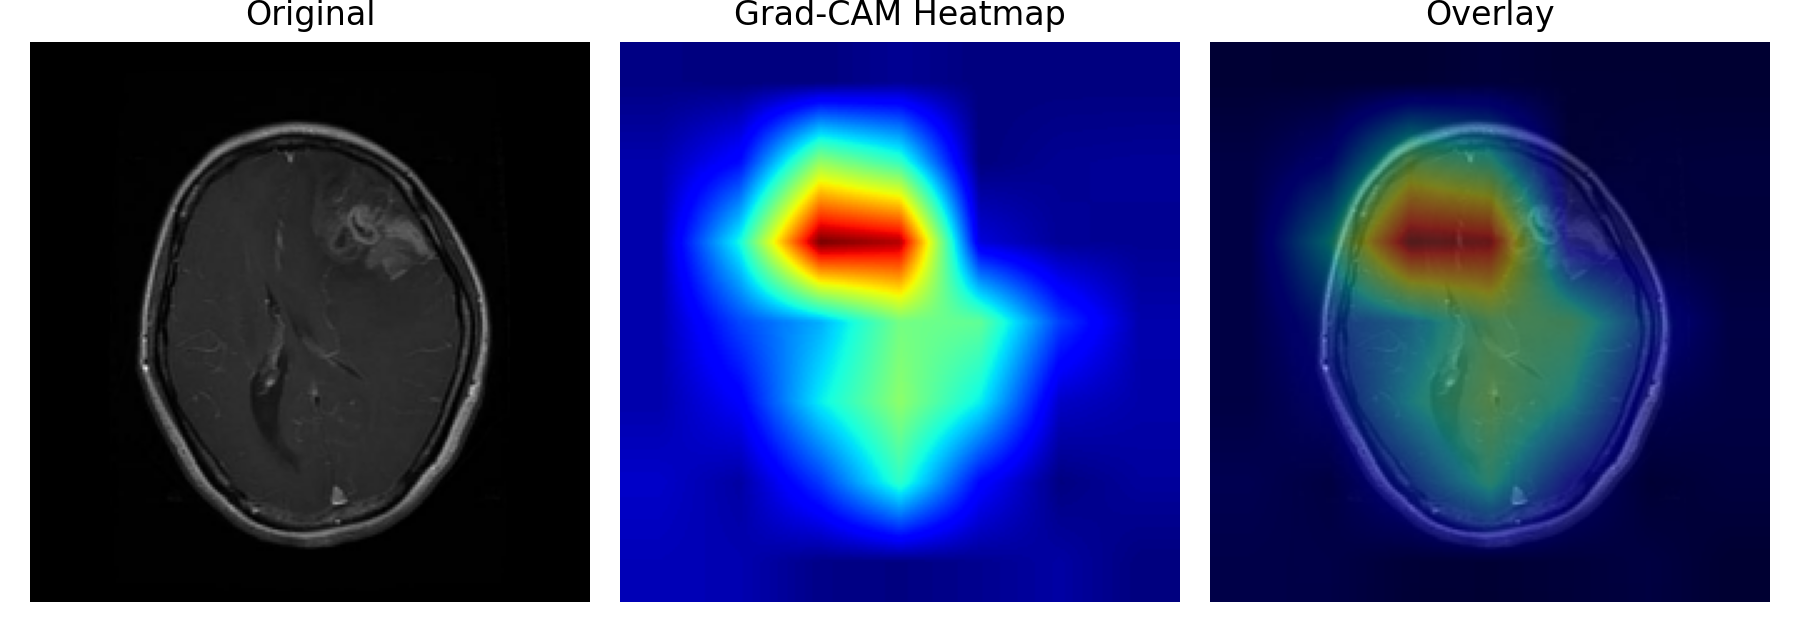
\includegraphics[width=\linewidth]{images/gradcam_glioma_0_correct.png}
\caption{Glioma}
\end{subfigure}
\begin{subfigure}[t]{0.48\linewidth}
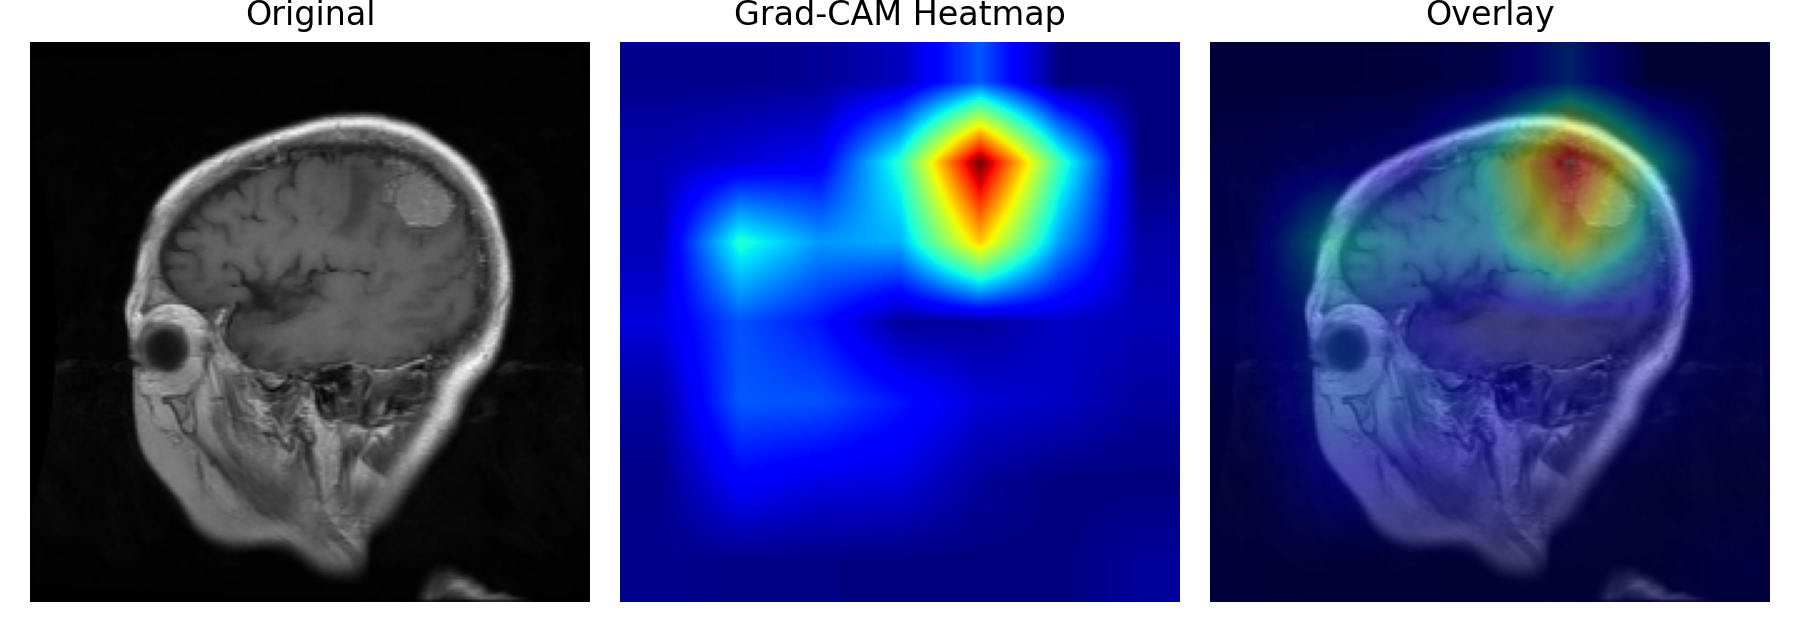
\includegraphics[width=\linewidth]{images/gradcam_meningioma_0_correct.png}
\caption{Meningioma}
\end{subfigure}

\begin{subfigure}[t]{0.48\linewidth}
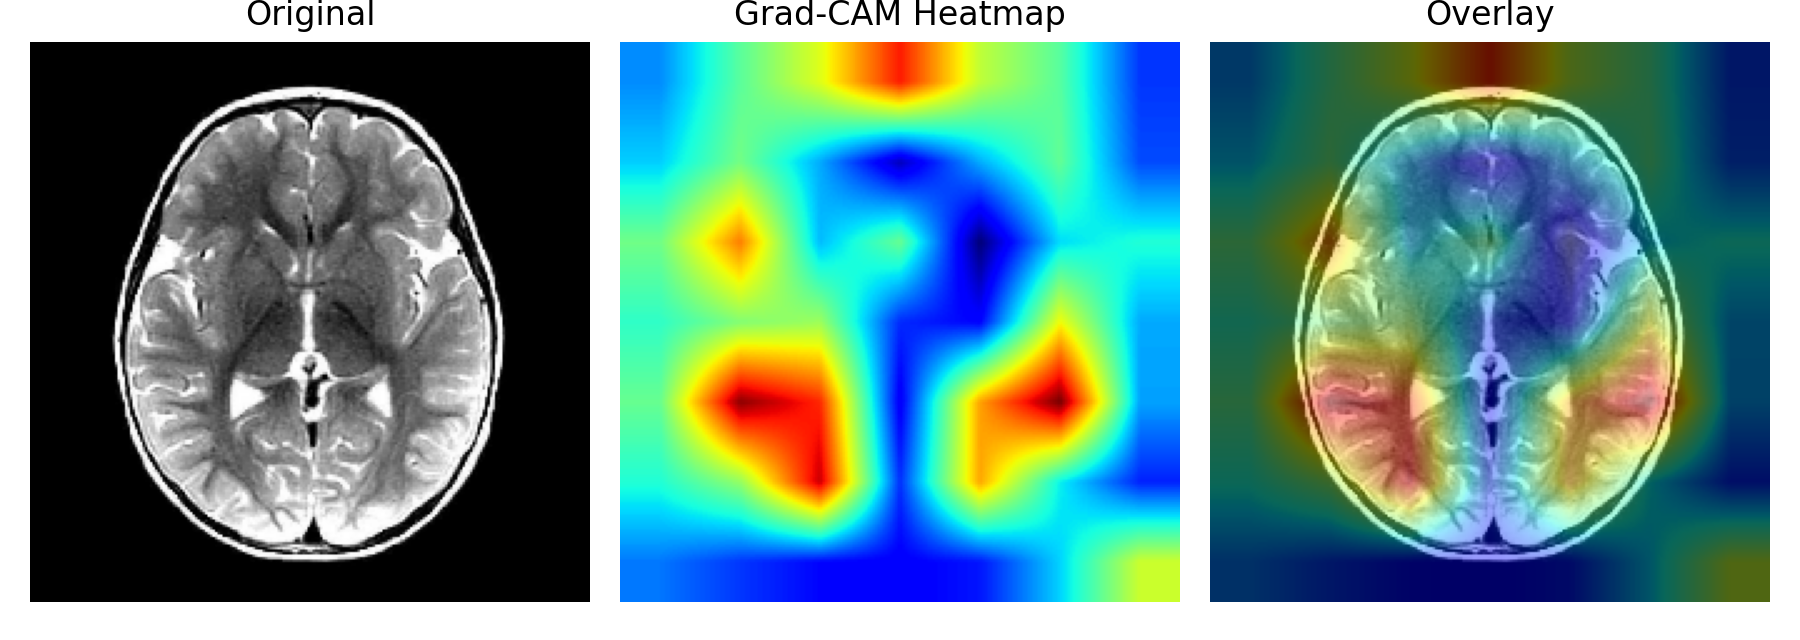
\includegraphics[width=\linewidth]{images/gradcam_notumor_0_correct.png}
\caption{No Tumor}
\end{subfigure}
\begin{subfigure}[t]{0.48\linewidth}
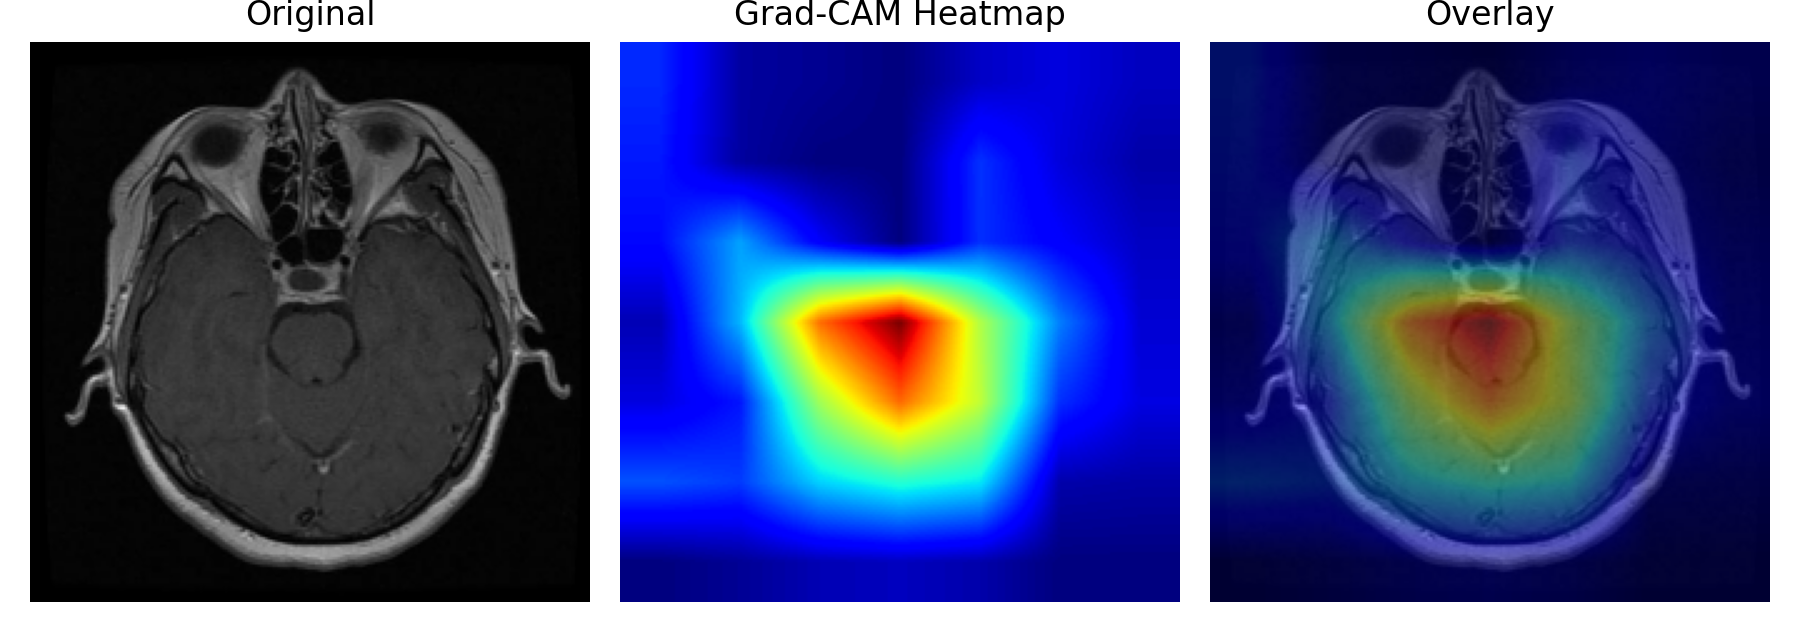
\includegraphics[width=\linewidth]{images/gradcam_pituitary_0_correct.png}
\caption{Pituitary Tumor}
\end{subfigure}
\caption{Grad-CAM visualizations (original, heatmap, overlay) for one correctly classified example per class. The model's attention (red regions) localizes to the visible mass for glioma and meningioma, to the sellar/skull-base region where the pituitary gland is located for pituitary tumor, and shows a diffuse, non-focal pattern for no-tumor cases.}
\label{fig:gradcam}
\end{figure}

The glioma heatmap closely matches the visibly abnormal tissue in the upper part of the slice. The meningioma heatmap is even more focused, concentrating on a well-defined mass next to the skull, which matches how meningiomas typically appear, since they grow attached to the dura outside the brain tissue. For pituitary tumor, even though the gland is small relative to the whole slice, the heatmap still concentrates on the sellar region at the skull base, which is the correct anatomical location. For no-tumor cases, there is no single hot spot; activation is spread out fairly evenly across both hemispheres, which is expected since there is no tumor for the model to focus on. Overall, these results suggest that the network is focusing on relevant anatomy rather than unrelated patterns in the image. However, Grad-CAM's resolution is limited since it comes from a heavily downsampled feature map, so it cannot show precise tumor boundaries, and we did not measure the overlap between the heatmap and the lesion quantitatively in this study, nor did we repeat this analysis for the other three backbones.

\subsection{Discussion}
\label{sec:discussion}

Two findings, taken together, shape how we would interpret this pipeline's accuracy. First, the choice of backbone matters, but less than the choice of inference strategy: switching from EfficientNetB0 to DenseNet121 or ResNet50 gains 0.6 percentage points on CNN+TTA accuracy, and does so consistently enough to be statistically significant for both ($p=0.031$ each, a clean sweep of all five folds), whereas adding TTA to a fixed backbone gains anywhere from 0.6 points (DenseNet121, whose raw CNN was already strong) to 2.9 points (MobileNetV2, whose raw CNN was the weakest of the four) -- significant for every backbone we tested, but of a size that depends heavily on how good the backbone already was without TTA. A practitioner with a fixed, already-strong backbone in production would likely get comparable value from either change; a practitioner with a weaker or lighter backbone would get more value from adding TTA than from a backbone swap. Second, the embedding ensemble is consistently competitive with, but not consistently better than, CNN+TTA, and its advantage over the plain CNN is statistically robust for three of the four backbones but not for DenseNet121, whose already-strong CNN leaves the ensemble's fold-wise advantage too inconsistent in direction for five folds to distinguish from chance.

The confusion patterns are consistent across backbones: meningioma varies a lot in appearance on imaging and does not always have clear boundaries, which explains why it was the class most often confused with glioma and pituitary tumor in every configuration we tested, while no-tumor, having no lesion to be confused with, was the easiest class everywhere.


\section{Limitations}
\label{sec:limitations}
Several factors limit how much these results should be trusted. The dataset does not include a patient ID field, so cross-validation is performed at the image level; near-duplicate images could end up on both sides of a fold, especially since the dataset itself is a merge of several public sources. This is a form of subject-level leakage, which has been identified as a common and often unaddressed source of inflated performance in medical imaging machine learning \cite{varoquaux2022leakage}. We do not have a patient-identified version of this same dataset, so we cannot directly measure how much, if any, of the reported accuracy is affected by this; a dataset that combined this dataset's scale and class taxonomy with recorded patient identifiers would let this question be tested as a controlled experiment, rather than left as an open concern.

The dataset snapshot used in this study (7,200 images, exactly 1,800 per class) differs from the 7,023-image, imbalanced-no-tumor-class composition reported for the same Kaggle dataset identifier by some prior works we compare against in Section~\ref{sec:sota} (Section~\ref{sec:eda}). We cannot confirm whether this reflects the dataset owner updating the release at some point between when those studies downloaded it and when we did, or some other difference in how the data was obtained; either way, our benchmarking comparison should be read as using the same publicly available dataset identifier rather than a byte-for-byte identical set of images. The exploratory analysis in Section~\ref{sec:eda} additionally shows that images within a class are not all the same MRI acquisition plane, and that at least one no-tumor example is a CT scan rather than an MRI slice, which qualifies the description of the dataset as uniformly T1-weighted MRI. Finally, the no-tumor class is both visibly brighter on average and more consistently framed than the tumor classes (Section~\ref{sec:eda}); we cannot rule out that this contributes to no-tumor's consistently strong classification performance alongside, or instead of, its clinical distinctiveness.

The multi-backbone comparison (Section~\ref{sec:backbone_results}) was run once per backbone; we did not repeat the Grad-CAM analysis for ResNet50, DenseNet121, or MobileNetV2, due to the additional GPU time each full backbone run requires (Section~\ref{sec:efficiency} shows a single backbone's 5-fold run costs 1.5-2.5 GPU-hours). It is possible that the Grad-CAM attention patterns differ by backbone; we have no evidence either way. We also did not run a component-wise ablation isolating the individual contributions of class weighting and the training-time augmentation policy, since both were part of the pipeline from the outset for every backbone tested.

The Wilcoxon signed-rank tests in Section~\ref{sec:stats_results} are limited by the small number of folds: with $n=5$, the smallest attainable one-sided $p$-value is $1/32 \approx 0.031$, so a comparison can only ever report ``significant at $\alpha=0.05$'' when one configuration wins every single fold; anything less than a clean sweep (e.g., MobileNetV2's 3-of-5 record against EfficientNetB0, Section~\ref{sec:stats_results}) cannot reach significance at this sample size regardless of how large the underlying effect might be. These tests should be read as evidence about consistency of direction across folds, not as precise estimates of effect size or a stand-in for a larger, independent replication.

A related limitation is run-to-run variance beyond what the fold-wise standard deviations capture: two independent runs of the identical EfficientNetB0 configuration (fixed random seed, identical code) produced 5-fold mean accuracies that agreed to within 0.1 percentage points overall but differed by up to 0.4 points on individual folds (Section~\ref{sec:cv_protocol}), consistent with known GPU-level non-determinism in certain cuDNN kernels. This means the fold-to-fold standard deviations reported throughout this paper likely understate the true uncertainty in these accuracy estimates by a small amount, since they do not include this additional source of variance; we did not repeat this reproducibility check for the other three backbones.

In addition, this study performs 2D slice classification rather than full 3D volumetric analysis, which is a simplification relative to standard radiological practice. Finally, since all the data comes from a limited set of source institutions and scanners, it is unclear how well this pipeline would perform on MRI acquired at other hospitals or on other equipment. These gaps motivate the future work outlined in Section~\ref{sec:futurework}.


\section{Ethical Considerations}
\label{sec:ethics}
This study relies exclusively on a publicly available, de-identified MRI dataset (Section~\ref{sec:datasets}); it did not involve direct interaction with human participants and did not require institutional ethical review or informed consent beyond what the original dataset publisher obtained. Despite the accuracy levels reported here, any deployment of a model like this in a clinical or screening context should be treated strictly as a decision-support aid for a qualified radiologist or clinician, not as a diagnostic replacement; final diagnostic decisions should remain under clinical supervision and be confirmed through standard protocols. The dataset used here originates from a limited set of source institutions and scanner types (Section~\ref{sec:limitations}), and does not include demographic metadata (age, sex, ethnicity) that would allow a fairness or subgroup-performance audit; we therefore cannot rule out uneven performance across patient subgroups not represented in the training data, and we recommend such an audit, alongside external validation on data from additional institutions, before any deployment beyond a research setting.


\section{Conclusion}
\label{sec:conclusion}
This paper evaluated a hybrid brain tumor classification pipeline -- two-stage backbone fine-tuning, class-weighted training, test-time augmentation, and a Random Forest/XGBoost/SVM embedding ensemble -- across four backbone architectures under a single, identical 5-fold cross-validation protocol, rather than reporting a single accuracy figure for a single configuration. On a four-class, 7,200-image dataset, the best configuration (ResNet50+TTA) reached 98.38\% $\pm$ 0.23\% mean accuracy across 5 folds, with DenseNet121 close behind; both beat the original EfficientNetB0 backbone in every one of the five folds tested ($p=0.031$ each). The lightweight MobileNetV2 reached a competitive 97.96\% -- itself ahead of EfficientNetB0's 97.75\% -- at 14-31\% lower training cost than the other three backbones and the lowest inference latency of the four. An exact Wilcoxon signed-rank test confirmed that TTA's improvement over the plain CNN softmax output is statistically significant for every backbone tested, and that the embedding ensemble's improvement is significant for three of the four backbones. We present these results, together with the limitations discussed in Section~\ref{sec:limitations}, as evidence for treating multi-backbone comparison and explicit statistical testing as standard practice in this literature, rather than as a claim that any single configuration reported here represents a definitive state-of-the-art result.


\section{Future Work}
\label{sec:futurework}
Several directions follow directly from the limitations above. Repeating the Grad-CAM analysis for ResNet50, DenseNet121, and MobileNetV2 (not only EfficientNetB0) would show whether the attention patterns reported here are backbone-general or backbone-specific. Identifying or annotating patient identifiers for this dataset, or evaluating on an equivalent dataset that already records them, would allow the leakage concern raised in Section~\ref{sec:limitations} to be tested directly rather than left as an open concern. A component-wise ablation isolating class weighting and the augmentation policy, alongside the backbone and TTA/ensemble comparisons already reported here, would complete the picture of which pipeline components drive the reported gains. Multi-scale feature fusion or additional attention mechanisms in the backbone may help specifically with boundary-ambiguous cases like meningioma, which caused the most errors in every configuration in this study. A CNN--Transformer hybrid or a newer state-space (Mamba-style) architecture is another backbone family not explored here. For interpretability, a quantitative evaluation -- measuring the overlap between the Grad-CAM heatmap and an annotated lesion mask, on a dataset that provides one -- would provide stronger evidence than visual inspection alone. Finally, this pipeline has not been tested on MRI from institutions outside this dataset's source, so external validation is a necessary next step before any of these configurations could be considered for clinical use.


\section*{Declarations}

\noindent\textbf{Ethics Approval and Consent to Participate:} Not applicable. This research uses two publicly available, de-identified MRI datasets and does not involve direct interaction with human participants or animals.

\noindent\textbf{Conflict of Interest:} The authors have no relevant financial or non-financial interests to disclose.

\noindent\textbf{Funding:} The authors declare that no funds, grants, or other external support were received during the preparation of this manuscript.

\noindent\textbf{Data Availability:} The four-class, 7,200-image benchmark used in this study is publicly available via Kaggle.

\noindent\textbf{Code Availability:} The source code used to run the experiments in this study is available from the corresponding author upon reasonable request.

\noindent\textbf{Author Contributions:} \textbf{Md Al Amin Tokder Shoukhin:} Conceptualization, Methodology, Software, Writing -- Original Draft Preparation. \textbf{Tasmia Jannat:} Methodology, Software, Data Curation. \textbf{Md. Ali Hossain:} Methodology, Formal Analysis, Validation. \textbf{Nazmul Haque:} Writing -- Review and Editing, Validation. All authors read and approved the final manuscript.

\bibliographystyle{ieeetr}
\bibliography{reference}
\end{document}
